

\documentclass[12pt, twoside, a4paper]{book}
%\documentclass[a4paper,12pt]{report}

% Contenido del preámbulo del documento LaTeX

\usepackage[utf8]{inputenc}
\usepackage{color}
\usepackage{tabulary}
\usepackage[table]{xcolor}
\usepackage[T1]{fontenc}		% Para poner los símbolos << y >>
\usepackage{setspace}
\usepackage{pstricks}
\usepackage{fancyhdr}
\usepackage{tocbibind}			% Incluye bibliografía en índice
\usepackage{natbib}
\bibliographystyle{unsrt}		% Estilo de la bibliografía.
\usepackage{fancyvrb}			% Para usar Verbatim
\usepackage{bookmark}			% Para insertar la bibliografía al mismo nivel que el resto de capítulos.
\usepackage{textcomp} 			% Para usar \textquotesingle
\usepackage{pdfpages}
\usepackage{epstopdf}
\usepackage{tikz} 				% Para posicionar imágenes.
\usepackage{gensymb} 			% Para poner el símbolo de los grados.

\usepackage{changepage}			% Para usar {adjustwidth}
\usepackage{tocbibind}			% Incluye bibliografía en índice

\usepackage{indentfirst}		% Indenta el primer párrafo de cada sección.

\usepackage{lineno}
\usepackage{caption}
\usepackage{appendix}

\usepackage{tcolorbox}

% Macro para los mensajes de tipo Warning.
\newtcolorbox{warningbox}[2]
{
	title = \textbf{#1},
	text width=#2,
	colback=red!4!white,
	colframe=orange!65!white
}

% Color gris para las filas de la tabla.
\definecolor{gray090}{gray}{0.90}

% Carpeta en la que se crean los .pdf a partir de las imágenes .eps
\epstopdfsetup{outdir=./figures_converted_to_pdf/}

\DeclareGraphicsExtensions{.eps}


% Espaciado de párrafo.
\parskip=5pt


% Indentación a la izquierda en cada comienzo de párrafo.
\parindent=30pt


% Márgenes del documento.
\usepackage[left=3.5cm, right=2.5cm, top=2.5cm, bottom=3.5cm]{geometry}


% Configuración del formato para la cabecera de los títulos.
\makeatletter
\def\LigneVerticale{\vrule height 4cm depth 2cm\hspace{0.1cm}\relax}

\def\LignesVerticales{%
  \let\LV\LigneVerticale\LV\LV\LV\LV\LV\LV\LV\LV\LV\LV}
  
\def\GrosCarreAvecUnChiffre#1{%
  \rlap{\vrule height 0.8cm width 1cm depth 0.2cm}%
  \rlap{\hbox to 1cm{\hss\mbox{\white #1}\hss}}%
  \vrule height 0pt width 1cm depth 0pt}
  
\def\@makechapterhead#1{\hbox{%
    \huge
    \LignesVerticales
    \hspace{-0.5cm}%
    \GrosCarreAvecUnChiffre{\thechapter}
    \hspace{0.4cm}\hbox{#1}%
}\par\vskip 2cm}

%\def\@makeschapterhead#1{\hbox{%
%    \huge
%    \LignesVerticales
%    \hspace{0.5cm}
%    \hbox{#1}%
%}\par\vskip 2cm}



% Configuración del formato de cabecera y pie de página.
\pagestyle{fancy}
\fancyhf{}							% Elimina la configuración actual de la cabecera.
\fancyfoot{}						% Elimina la configuración actual del pie de página.
\fancyhead[LO]{\leftmark}	 	% Páginas impares ........: en la parte izquierda del encabezado aparecerá el nombre del capítulo.
\fancyhead[RE]{\rightmark}	 	% Páginas pares ..........: en la parte derecha del encabezado aparecerá el nombre de la sección.
\fancyfoot[RO,LE]{\thepage} 	% Númeración de páginas ..: impares en la derecha, pares en la izquierda.


% Para no incluir el encabezado en páginas en blanco.
\makeatletter
  \def\cleardoublepage{\clearpage\if@twoside \ifodd\c@page\else
  \vspace*{\fill}
    \thispagestyle{empty}
    \newpage
    \if@twocolumn\hbox{}\newpage\fi\fi\fi}
\makeatother


% Comando para insertar una página vacía completa.
\newcommand{\paginavaciacompleta}{\newpage{\thispagestyle{empty}\cleardoublepage}}


\hyphenation{matching}



\begin{document}

	% Formato para el capítulo: N. Nombre
	\renewcommand{\chaptermark}[1]{\markboth{\textbf{\thechapter. #1}}{}}

	% Formato para la sección: N.M. Nombre
	\renewcommand{\sectionmark}[1]{\markright{\textbf{\thesection. #1}}}

	% Ancho de la línea horizontal bajo el encabezado
	\renewcommand{\headrulewidth}{0.6pt}

	% Aumenta la altura del encabezado en 1.5 veces.
	\setlength{\headheight}{1.5\headheight}
	
	
	% Unidades frontales del book
	% Emplea numeración con números romanos
	\frontmatter

	% Portada
	
\thispagestyle{empty}


	\begin{tikzpicture}[remember picture,overlay]

		%Logo.
		\node[xshift=10.6cm,yshift=19cm] at (current page.south west)
					{
\includegraphics[scale=0.75]{figures/logo.png}};

	\end{tikzpicture}
	
	\vspace{10.0cm}
	
	\textbf{\Large SPAMDA}
	
	\vspace{0.25cm}
		
	\textit{\Large Software for Pre-processing and Analysis of}
	
	\textit{\Large Meteorological DAta to build datasets.}
	
	\vspace{6.0cm}
	
	\textit{SPAMDA 1.0v User manual}


	% Página en blanco
	\newpage
	
	% Página con el copyright de la documentación.
	

\thispagestyle{empty}

\small

\vspace*{\fill} % El texto aparecerá en la parte inferior de la página.

\begin{quote}

	SPAMDA: Software for Pre-processing and Analysis of Meteorological DAta to build datasets.

	This is the version 1.0 of the SPAMDA manual.

	Copyright (c) 2017-2018 by AYRNA Research Group. https://www.uco.es/ayrna/

	\hspace{1.005cm}Authors:

	\hspace{1.30cm}Antonio Manuel Gómez Orellana, Juan Carlos Fernández Caballero,

	\hspace{1.30cm}Manuel Dorado Moreno, Pedro Antonio Gutiérrez Peña and 

	\hspace{1.30cm}César Hervás Martínez.

	\begin{quote} % El texto aparecerá con un margen izquierdo y derecho de 1cm.
		Permission is granted to copy, distribute and/or modify this document 
		under the terms of the GNU Free Documentation License, Version 1.3 or any later
		version published by the Free Software Foundation; with no Invariant Sections, 
		with no Front-Cover Texts, with the Front-Cover logo, and with no Back-Cover Texts.
		\newline
		\newline
		A copy of the license is included in the appendix entitled "GNU Free Documentation License" \ref{GFDL_LICENSE}. If not, see <http://www.gnu.org/licenses/>.

		\vspace{0.50cm}
		Contact information:
	
		\begin{quote}
			Juan Carlos Fernández Caballero, PhD.

			email: jfcaballero@uco.es

			Address: University of Córdoba, Department of Computer Science and Numerical Analysis, Rabanales Campus, AYRNA Research Group, Einstein Building, 3rd floor. Road Madrid-Cádiz, Km 396-A. 14071 - Córdoba (Spain)
		\end{quote}

	\end{quote}

\end{quote}












	% Índice de contenido
	\tableofcontents
	
	% Página en blanco
	\paginavaciacompleta

	% Índice de figuras
	\listoffigures
	
	% Página en blanco
	\paginavaciacompleta

	% Índice de tablas
	\listoftables
	
	% Página en blanco
	%\paginavaciacompleta
	
	% Unidad principal del book
	% Comienza numeración capítulos y numeración arábiga de las páginas.
	\mainmatter


	% Nueva página
	\newpage
	
	%\part{User manual}

	
\chapter{Introduction to SPAMDA}

	\begin{onehalfspace}

		\section{SPAMDA description}

			SPAMDA is a software tool for creating datasets with meteorological data from two well-known sources of information, \textit{National Data Buoy Center} (NDBC) \cite{NOAA} and \textit{Reanalysis Project} (NNRP or R1) \cite{Kalnay1996, Kistler2001}.
			
			The datasets created with SPAMDA will be ready to use as input for Machine Learning (ML) techniques in classification or regression prediction tasks, although the researchers may use them in the way they deem suitable. These datasets will contain one or more meteorological variables as inputs and another one as target (variable to predict). The format of the datasets will be \textit{Attribute-Relation File Format} (ARFF) \cite{WEKA_ARFF} that it is used by the well-known tool \textit{Waikato Environment for Knowledge Analysis} (WEKA) \cite{WEKA}, which provides a wide collection of ML algorithms. Besides, the datasets can also be generated in \textit{Comma-Separated Values} (CSV) format, enabling the researchers to use others tools.
			
			Some of the advantages that SPAMDA tool offers are briefly summarised below:

				\begin{itemize}
					\item The generation of datasets becomes a very easy and customizable task, by means of the selection of different input parameters.
					\item It makes the researcher focus on oceanic and atmospheric studies, without having to worry about mechanical tasks.
					\item It provides information about the quality and quantity of the data.
					\item It avoids possible researcher errors in the intermediate steps of the process of creation of the datasets.
					\item It includes different pre-processing tasks, such as normalisation and missing data recovery.
					\item It facilitates data management and well-organised storage of the datasets.
					\item Its modular design allows the implementation of new functional modules for managing meteorological data from others sources for renewable energy research.
					\item It includes an user-friendly GUI, facilitating and greatly simplifying data management, and it is integrated with the Explorer environment of WEKA.
					\item It is multi-platform, and it can be used on any computer with Java regardless of the operating system.
				\end{itemize}
				
	\section{Meteorological data sources}\label{sec:DataSources}
		
		The data provided by the above-mentioned sources of information used by SPAMDA is briefly described below:
		
		\begin{itemize}

			\item NDBC is a part of the \textit{National Weather Service} (NWS). NDBC designs, develops, operates, and maintains a network of data collecting buoys (stations). The mission of the network is to collect real-time marine meteorological and oceanographic observations, such as wave height, dominant wave period, or wind speed and direction, among others.

			The buoys maintained by NDBC are deployed in the coastal and offshore waters around oceans and seas, and are equipped with assorted sensors which allow them to perform different measurements. The information collected by the buoys is available in NDBC web page \cite{NOAA_1}, which is divided into different groups. One of them is the standard meteorological information of the historical data collected by each buoy, which can be downloaded as annual text files and whose format was adopted by NDBC since January 2007 \cite {NOAA_2}. These files contain hourly measurements per day from $00$:$50$ to $23$:$50$ UTC and from $23$:$50$ 31th Dec of the previous desired year to $22$:$50$ 31th Dec of the desired year. In Table \ref{tab:measurementsDescription} a comprehensive measurements descriptions and units of such information is provided.
			
			\clearpage
			
			\begin{table}[ht!]
			
				\caption{Measurements descriptions and units of each meteorological variable or attribute collected by the buoys.}
				\label{tab:measurementsDescription}
				\footnotesize
				\centering
				
				\begin{tabular}{ccm{11.00cm}@{\setlength{\tabcolsep}{0pt}}m{0.0cm}}
				
					\cline{1-4}
					
					%\textbf{Variable}&\textbf{Units}&\textbf{Description}&\\[0.30cm]
					
					\textbf{Attribute}&\textbf{Units}&\textbf{Description}&\\[0.30cm]
 
					\cline{1-4}
					
					WDIR & degT & Wind direction (the direction the wind is coming from in degrees clockwise from true N) during the same period used for WSPD. \\
					
					\cellcolor{gray090}WSPD & \cellcolor{gray090} m/s & \cellcolor{gray090} Wind speed (m/s) averaged over an eight-minute period for buoys and a two-minute period for land stations. Reported Hourly. \\
					
					GST &  m/s & Peak 5 or 8 second gust speed (m/s) measured during the eight-minute or two-minute period. \\
					
					\cellcolor{gray090} WVHT & \cellcolor{gray090} m & \cellcolor{gray090} Significant wave height (meters) is calculated as the average of the highest one-third of all of the wave heights during the 20-minute sampling period. \\
					
					DPD & sec & Dominant wave period (seconds) is the period with the maximum wave energy. \\
					
					\cellcolor{gray090}APD & \cellcolor{gray090} sec & \cellcolor{gray090} Average wave period (seconds) of all waves during the 20-minute period. \\
					
					MWD & degT & The direction from which the waves at the dominant period (DPD) are coming. The units are degrees from true North, increasing clockwise, with North as 0 (zero) degrees and East as 90 degrees. \\
					
					\cellcolor{gray090}PRES & \cellcolor{gray090} hPa & \cellcolor{gray090} Sea level pressure (hPa). For C-MAN sites and Great Lakes buoys, the recorded pressure is reduced to sea level using the method described in NWS Technical Procedures Bulletin 291 (11/14/80). \\
					
					ATMP & degC & Air temperature (Celsius). &\\[0.10cm]
					
					\cellcolor{gray090}WTMP & \cellcolor{gray090} degC & \cellcolor{gray090} Sea surface temperature (Celsius). For buoys the depth is referenced to the hull's waterline. For fixed platforms it varies with tide, but is referenced to, or near Mean Lower Low Water (MLLW).\\
					
					DEWP & degC & Dewpoint temperature taken at the same height as the air temperature measurement. \\
					
					\cellcolor{gray090}VIS & \cellcolor{gray090} nmi & \cellcolor{gray090} Station visibility (nautical miles). Note that buoy stations are limited to reports from 0 to 1.6 nmi. \\
					
					%PTDY & hPa & Pressure Tendency is the direction (plus or minus) and the amount of pressure change (hPa) for a three hour period ending at the time of observation. \\
					
					TIDE & ft & The water level in feet above or below Mean Lower Low Water (MLLW). \\
					
					\cline{1-4}
						
				\end{tabular}
			 
			\end{table}

			
			\item NNRP provides three-dimensional global reanalysis of numerous meteorological variables (e.g. air temperature, U/V-wind, relative humidity, pressure, etc.), which is available monthly, daily and every $6$ hours at $00$Z, $06$Z, $12$Z and $18$Z from $1948$ on a global $2.5\degree$ x $2.5\degree$ grid. Weather observations are from different sources, such as ships, satellites and radar, among others.
			
			%The reanalysis data is available in NNRP web page \cite{NNRP}, which are accessible through the different sections. Such data can be fully (a global $2.5\degree$ x $2.5\degree$ grid) or partially (only the desired reanalysis nodes or sub-grid) downloaded as \textit{Network Common Data Form} (NetCDF) files \cite{NetCDF}, a special binary format for representing scientific data which provides a description of what the data in each variable represents and the spatial and temporal properties of the data. Each reanalysis data file contains the estimated values by a mathematical model of one meteorological variable and for each reanalysis node. For a better understanding, in Fig. \ref{fig:subGrid} an approximate representation of a six sub-grid reanalysis nodes around the geographical localisation of a buoy (obtained from NDBC) is shown.
			
			The reanalysis data is available in NNRP web page \cite{NNRP}, which are accessible through the different sections. Such data can be fully (a global $2.5\degree$ x $2.5\degree$ grid) or partially (only the desired reanalysis nodes or sub-grid) downloaded as \textit{Network Common Data Form} (NetCDF) files \cite{NetCDF}, a special binary format for representing scientific data which provides a description of the file contents and also includes the spatial and temporal properties of the data. Each reanalysis file contains the values of a meteorological variable estimated by a mathematical model for each reanalysis node. For a better understanding, in Fig. \ref{fig:subGrid} an approximate representation of a sub-grid containing six reanalysis nodes around the geographical localisation of a buoy (obtained from NDBC) is shown.
			
			\begin{figure}[ht!]
				\centering
				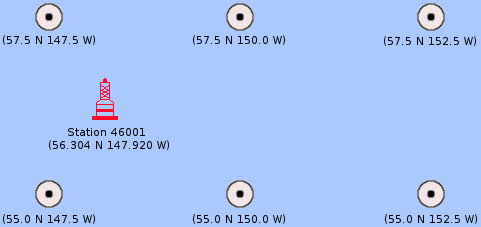
\includegraphics[scale=0.52]{figures/FigureSubGrid.jpg}
				\caption{Example of a six sub-grid reanalysis nodes around the \textit{Station 46001}.}
				\label{fig:subGrid}
			\end{figure}
			
		\end{itemize}
		
		With both sources of information SPAMDA will create datasets for prediction tasks. In this way, the input variables of the dataset will be one or more reanalysis variables from NNRP and one or more measurements from NDBC. The output variable of the dataset will be one measurement from NDBC. Note that the output variable cannot be used as input also.

	\end{onehalfspace}

	
\chapter{Getting started}

	\begin{onehalfspace}

		\section{System requirements}

			%SPAMDA has been developed in Java, therefore it is a multi-platform software tool. In this way, any computer able to install and run a Java Virtual Machine (JVM) will be enough for running the developed tool.
			
			SPAMDA has been developed in Java, therefore it is a multi-platform software tool. In this way, any computer having Java Virtual Machine (JVM) installed would be able to run the developed tool.
			
			As SPAMDA has been compiled for Java JRE 1.8v, Java version 8 needs to be installed in the system, which can be downloaded from \cite{Java} choosing the correct distribution depending on the system platform.
			
		\section{Installing SPAMDA}
		
			The process of installation of SPAMDA is quite easy and it does not require administrator permissions to carry it out. The following sections describe how to perform the installation process according to the system platform.
			
			\subsection{Installing on Linux}
			
				To install SPAMDA on Linux follow the next steps:
			
					\begin{itemize}
						\item \textit{\textbf{Step 1}}: Download the SPAMDA software on the computer.
						\item \textit{\textbf{Step 2}}: Create a folder and copy the downloaded file inside it.
						\item \textit{\textbf{Step 3}}: Decompress the file.
					\end{itemize}
					
				After performing the above steps SPAMDA would be installed on the computer and ready to be run. Note that the process of installation creates all the folders and files necessary inside the folder created in \textit{\textbf{Step 2}}. In Fig. \ref{fig:installationOnLinux} is represented an example of installation in the folder named ``SPAMDA'', which will contain the software tool.
				
				\begin{figure}[ht!]
					\centering
					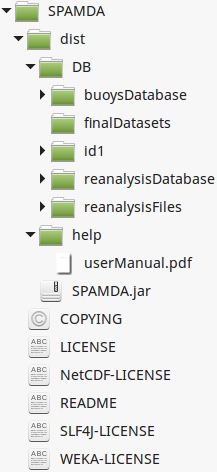
\includegraphics[scale=0.40]{figures/installationOnLinux.png}
					\caption{Content of the folder after installing SPAMDA (Linux).}
					\label{fig:installationOnLinux}
				\end{figure}
				
				Following, the structures of each folder and file created as a result of the installation are described:
				
					\begin{itemize}
						\item \textbf{\textit{dist}}: Contains the binary distribution of SPAMDA, which consist of:
							\begin{itemize}
								\item \textbf{\textit{DB}}: Contains all the information managed by SPAMDA.
									\begin{itemize}
										\item \textbf{\textit{buoysDatabase}}: Contains the database of the buoys.
										\item \textbf{\textit{finalDatasets}}: It is used as a default folder to save the final datasets.
										\item \textbf{\textit{id1}}: Contains the information of the buoy (annual text files, intermediate datasets, pre-processed datasets and matching configurations) entered as example.
										\item \textbf{\textit{reanalysisDatabase}}: Contains the database of the reanalysis data.
										\item \textbf{\textit{reanalysisFiles}}: Contains the reanalysis files entered through SPAMDA.
									\end{itemize}
								\item \textbf{\textit{help}}: Contains the user manual of SPAMDA.
									\begin{itemize}
										\item \textbf{\textit{userManual.pdf}}: This is the user manual.
									\end{itemize}
								\item \textbf{\textit{SPAMDA.jar}}: This is the runnable file containing SPAMDA.
							\end{itemize}
						\item \textbf{\textit{COPYING}}: This file contains a copy of the license of the GNU GENERAL PUBLIC LICENSE.
						\item \textbf{\textit{LICENSE}}: This file contains a copy of the license of SPAMDA.
						\item \textbf{\textit{NetCDF-LICENSE}}: This file contains a copy of the license of the Library NetCDF Java version 4.6.10
						\item \textbf{\textit{README}}: This file contains the instructions for getting started with SPAMDA.
						\item \textbf{\textit{SLF4j-LICENSE}}: This file contains a copy of the license of the Library SLF4J version 1.7.25
						\item \textbf{\textit{WEKA-LICENSE}}: This file contains a copy of the license of the Library WEKA version 3.8.1
					\end{itemize}
				
				After installing SPAMDA, and in order to run it, open the ``dist'' folder (as shown in Fig. \ref{fig:runningSPAMDAonLinux}) and type the following command on the command-line of the terminal:
				
				\texttt{java -jar SPAMDA.jar}
				
				\begin{figure}[ht!]
					\centering
					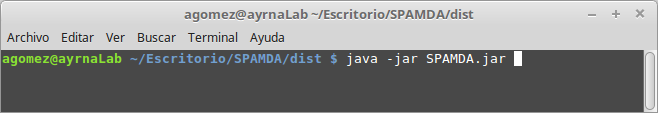
\includegraphics[scale=0.50]{figures/runningSPAMDAonLinux.png}
					\caption{Running SPAMDA on Linux.}
					\label{fig:runningSPAMDAonLinux}
				\end{figure}
				
				After executing such command, the main view of SPAMDA represented in Figure \ref{fig:SPAMDAmainViewonLinux} will appear.
				
				\begin{figure}[ht!]
					\centering
					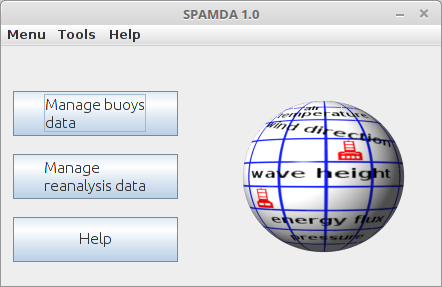
\includegraphics[scale=0.50]{figures/mainView.png}
					\caption{SPAMDA main view (Linux).}
					\label{fig:SPAMDAmainViewonLinux}
				\end{figure}

				
			\subsection{Installing on Windows}
			
				To install SPAMDA on Windows follow the next steps:
			
					\begin{itemize}
						\item \textit{\textbf{Step 1}}: Download the SPAMDA software on the computer.
						\item \textit{\textbf{Step 2}}: Create a folder and copy the downloaded file inside it.
						\item \textit{\textbf{Step 3}}: Decompress the file.
					\end{itemize}
					
				After performing the above steps SPAMDA would be installed on the computer and ready to be run. Note that the process of installation creates all the folders and files necessary inside the folder created in \textit{\textbf{Step 2}}. In Fig. \ref{fig:installationOnWindows} is represented an example of installation in the folder named ``SPAMDA'', which will contain the software tool.
				
				\begin{figure}[ht!]
					\centering
					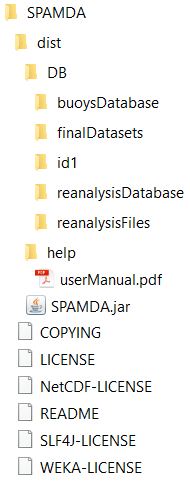
\includegraphics[scale=0.60]{figures/installationOnWindows.png}
					\caption{Content of the folder after installing SPAMDA (Windows).}
					\label{fig:installationOnWindows}
				\end{figure}
				
				Following, the structures of each folder and file created as a result of the installation are described:
				
					\begin{itemize}
						\item \textbf{\textit{dist}}: Contains the binary distribution of SPAMDA, which consist of:
							\begin{itemize}
								\item \textbf{\textit{DB}}: Contains all the information managed by SPAMDA.
									\begin{itemize}
										\item \textbf{\textit{buoysDatabase}}: Contains the database of the buoys.
										\item \textbf{\textit{finalDatasets}}: It is used as a default folder to save the final datasets.
										\item \textbf{\textit{id1}}: Contains the information of the buoy (annual text files, intermediate datasets, pre-processed datasets and matching configurations) entered as example.
										\item \textbf{\textit{reanalysisDatabase}}: Contains the database of the reanalysis data.
										\item \textbf{\textit{reanalysisFiles}}: Contains the reanalysis files entered through SPAMDA.
									\end{itemize}
								\item \textbf{\textit{help}}: Contains the user manual of SPAMDA.
									\begin{itemize}
										\item \textbf{\textit{userManual.pdf}}: This is the user manual.
									\end{itemize}
								\item \textbf{\textit{SPAMDA.jar}}: This is the runnable file containing SPAMDA.
							\end{itemize}
						\item \textbf{\textit{COPYING}}: This file contains a copy of the license of the GNU GENERAL PUBLIC LICENSE.
						\item \textbf{\textit{LICENSE}}: This file contains a copy of the license of SPAMDA.
						\item \textbf{\textit{NetCDF-LICENSE}}: This file contains a copy of the license of the Library NetCDF Java version 4.6.10
						\item \textbf{\textit{README}}: This file contains the instructions for getting started with SPAMDA.
						\item \textbf{\textit{SLF4j-LICENSE}}: This file contains a copy of the license of the Library SLF4J version 1.7.25
						\item \textbf{\textit{WEKA-LICENSE}}: This file contains a copy of the license of the Library WEKA version 3.8.1
					\end{itemize}
				
				After installing the software, and in order to run it, open the ``dist'' folder and double-click on the SPAMDA.jar file. Next, the main view of SPAMDA represented in figure \ref{fig:SPAMDAmainViewonWindows} will appear.
				
				\begin{figure}[ht!]
					\centering
					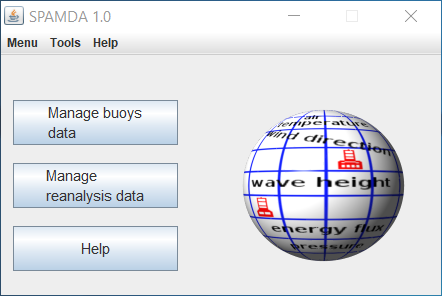
\includegraphics[scale=0.80]{figures/mainViewonWindows.png}
					\caption{SPAMDA main view (Windows).}
					\label{fig:SPAMDAmainViewonWindows}
				\end{figure}

			
			\subsection{Installing on macOS}
			
				To install SPAMDA on macOS follow the next steps:
			
					\begin{itemize}
						\item \textit{\textbf{Step 1}}: Download the SPAMDA software on the computer.
						\item \textit{\textbf{Step 2}}: Create a folder and copy the downloaded file inside it.
						\item \textit{\textbf{Step 3}}: Decompress the file.
					\end{itemize}
					
				After performing the above steps SPAMDA would be installed on the computer and ready to be run. Note that the process of installation creates all the folders and files necessary inside the folder created in \textit{\textbf{Step 2}}. In Fig. \ref{fig:installationOnMacOS} is represented an example of installation in the folder named ``SPAMDA'', which will contain the software tool.
				
				\begin{figure}[ht!]
					\centering
					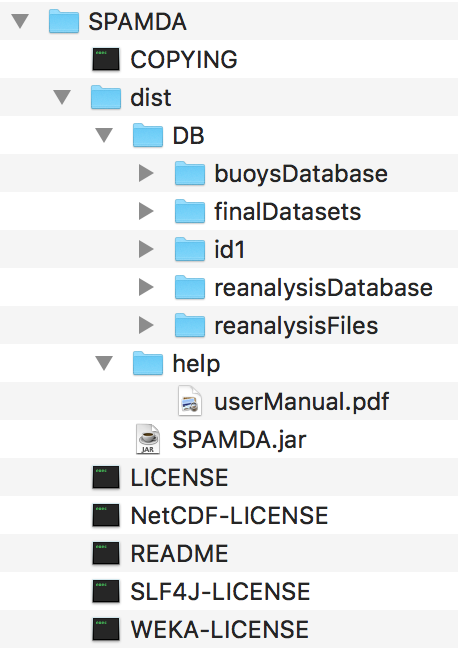
\includegraphics[scale=0.60]{figures/installationOnMacOS.png}
					\caption{Content of the folder after installing SPAMDA (macOS).}
					\label{fig:installationOnMacOS}
				\end{figure}
				
				Following, the structures of each folder and file created as a result of the installation are described:
				
					\begin{itemize}
						\item \textbf{\textit{dist}}: Contains the binary distribution of SPAMDA, which consist of:
							\begin{itemize}
								\item \textbf{\textit{DB}}: Contains all the information managed by SPAMDA.
									\begin{itemize}
										\item \textbf{\textit{buoysDatabase}}: Contains the database of the buoys.
										\item \textbf{\textit{finalDatasets}}: It is used as a default folder to save the final datasets.
										\item \textbf{\textit{id1}}: Contains the information of the buoy (annual text files, intermediate datasets, pre-processed datasets and matching configurations) entered as example.
										\item \textbf{\textit{reanalysisDatabase}}: Contains the database of the reanalysis data.
										\item \textbf{\textit{reanalysisFiles}}: Contains the reanalysis files entered through SPAMDA.
									\end{itemize}
								\item \textbf{\textit{help}}: Contains the user manual of SPAMDA.
									\begin{itemize}
										\item \textbf{\textit{userManual.pdf}}: This is the user manual.
									\end{itemize}
								\item \textbf{\textit{SPAMDA.jar}}: This is the runnable file containing SPAMDA.
							\end{itemize}
						\item \textbf{\textit{COPYING}}: This file contains a copy of the license of the GNU GENERAL PUBLIC LICENSE.
						\item \textbf{\textit{LICENSE}}: This file contains a copy of the license of SPAMDA.
						\item \textbf{\textit{NetCDF-LICENSE}}: This file contains a copy of the license of the Library NetCDF Java version 4.6.10
						\item \textbf{\textit{README}}: This file contains the instructions for getting started with SPAMDA.
						\item \textbf{\textit{SLF4j-LICENSE}}: This file contains a copy of the license of the Library SLF4J version 1.7.25
						\item \textbf{\textit{WEKA-LICENSE}}: This file contains a copy of the license of the Library WEKA version 3.8.1
					\end{itemize}
				
				After installing the software, and in order to run it, open the ``dist'' folder and double-click on the SPAMDA.jar file. Next, the main view of SPAMDA represented in figure \ref{fig:SPAMDAmainViewonMacOS} will appear.
				
				\begin{figure}[ht!]
					\centering
					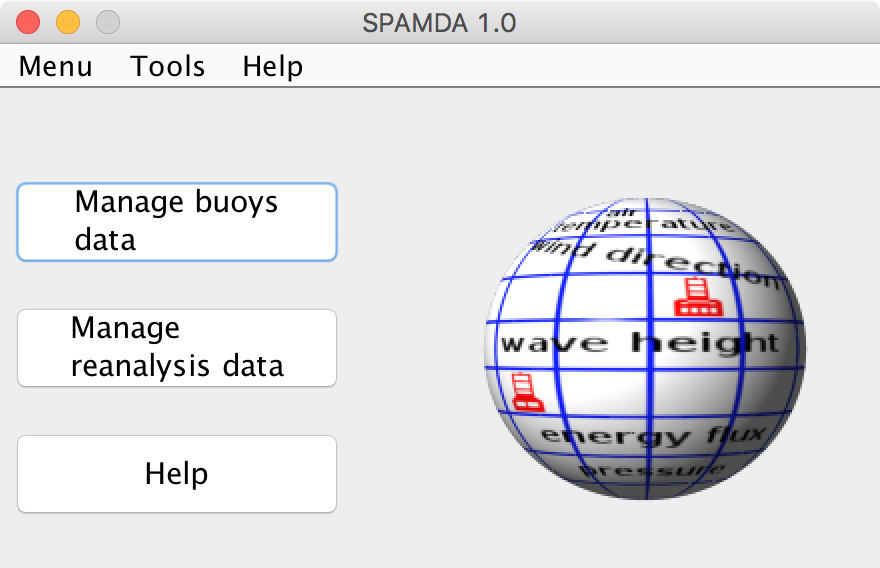
\includegraphics[scale=0.50]{figures/mainViewonMacOS.png}
					\caption{SPAMDA main view (macOS).}
					\label{fig:SPAMDAmainViewonMacOS}
				\end{figure}

			
		\section{How to uninstall?}
		
			To uninstall SPAMDA just delete the folder in which the installation process was carried out. 
			
			\begin{center}
				\begin{warningbox}{Warning}{13cm}
					This action will remove SPAMDA from your computer and any information entered in SPAMDA or generated by means of it will be lost.
				\end{warningbox}
			\end{center}

	\end{onehalfspace}

	
\chapter{Using SPAMDA}

	\begin{onehalfspace}
	
		SPAMDA has been designed to greatly simplify all the steps involved in the creation of datasets with information from the sources mentioned in Section \ref{sec:DataSources}, thus the researcher can create as different datasets of the same meteorological data as needed, in a quick and efficient manner. For this purpose, SPAMDA manages three different types of datasets that are briefly introduced bellow:
			\begin{itemize}
				\item \textit{Intermediate datasets}: Which will contain the meteorological observations from NDBC.
				\item \textit{Pre-processed datasets}: Obtained as a result of pre-processing tasks performed on the intermediate datasets.
				\item \textit{Final datasets}: Created by merging an intermediate or pre-processed dataset with the reanalysis data (referenced as matching process) and according to the needs of the study to perform (classification or regression).
			\end{itemize}
			
		SPAMDA consists of the following three main functional modules:
			\begin{itemize}
				\item \textbf{\textit{Manage buoys data}}
				\item \textbf{\textit{Manage reanalysis data}}
				\item \textbf{\textit{Tools}}
			\end{itemize}
			
		\begin{figure}[ht!]
			\centering
			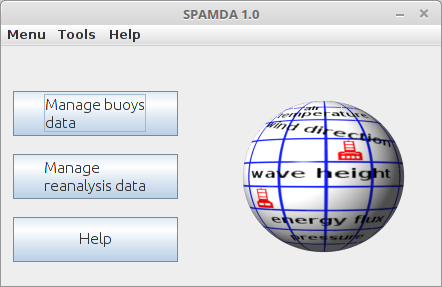
\includegraphics[scale=0.5]{figures/mainView.png}
			\caption{SPAMDA main view.}
			\label{fig:mainView}
		\end{figure}
			
		Such functional modules, which will be described in detail in the following sections, are accessible through the main view of SPAMDA represented in Fig. \ref{fig:mainView}.

		\section{Manage buoys data}

			The aim of this module is to provide the features for the management and analysis of the information related to the buoys from NDBC, since such information is entered in SPAMDA until it is used by the researchers for conducting their studies. Such management and analysis involves:
				\begin{itemize}
					\item Entering and updating the information of each buoy.
					\item The creation of the intermediate datasets with the collected measurements.
					\item Pre-processing tasks for obtaining the pre-processed datasets.
					\item The matching process to merge the information from NDBC and NNRP.
					\item The creation of the final datasets accordingly to the ML technique to use.
				\end{itemize}
				
			The following sections describe the organisation of this module.
			
			\subsection{Buoys}
			
				The \textit{Buoys} tab, which is represented in Fig. \ref{fig:tabBuoys}, allows the researchers to enter and update the information of each buoy. When entering a new buoy the following information, which can be obtained from NDBC, is requested:
				
				\begin{figure}[ht!]
					\centering
					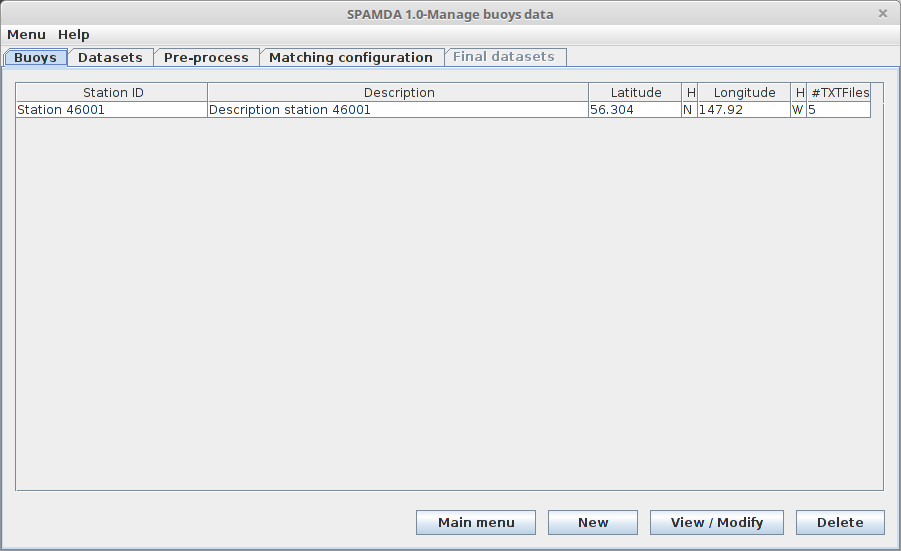
\includegraphics[scale=0.40]{figures/tabBuoys.png}
					\caption{Tab \textit{Buoys}.}
					\label{fig:tabBuoys}
				\end{figure}
				
				\begin{itemize}
					\item \textit{\textbf{Station ID}}: An alphanumeric identifier that allows the researchers to easily identify the buoy.
					\item \textit{\textbf{Description}}: A short description of the buoy.
					\item \textit{\textbf{Latitude}}: North or South geographical localisation (degrees) of the buoy. 
					\item \textit{\textbf{Longitude}}: West or East geographical localisation (degrees) of the buoy.
					\item \textit{\textbf{Measurements files}}: The above-mentioned annual text files of the standard meteorological information collected by the buoy and downloaded from NDBC web page, which will be used for the creation of the intermediate datasets. The researchers will add to the buoy one file per year and as many as needed. Remember that such files are available in NDBC web page \cite{NOAA_1}.
				\end{itemize}
				
				%To enter a new buoy click on \textcolor{blue}{\textit{New}} button, after typing the required information click on \textcolor{blue}{\textit{Save}} button for inserting the buoy. An example of entering a new boy is represented in Fig. \ref{fig:enteringBuoy}.
				
				To enter a new buoy follow the next steps:
				
					\begin{itemize}\itemsep0.02cm
						\item \textit{\textbf{Step 1}}: Click on the \textcolor{blue}{\textit{New}} button and the view represented in Fig. \ref{fig:enteringBuoy} will be displayed. (The remaining steps are related to such view).
						\item \textit{\textbf{Step 2}}: Type the required information about the buoy. To enter a new annual text file of the buoy click on the \textcolor{blue}{\textit{Add file}} button or click on the \textcolor{blue}{\textit{Delete file}} button to delete the selected one. By clicking on the \textcolor{blue}{\textit{Clear}} button it is possible to clean the form that request the information.
						\item \textit{\textbf{Step 3}}: Click on the \textcolor{blue}{\textit{Save}} button to insert the buoy.
					\end{itemize}
					
				%An example of entering a new boy is represented in Fig. \ref{fig:enteringBuoy}.
				
				\begin{figure}[ht!]
					\centering
					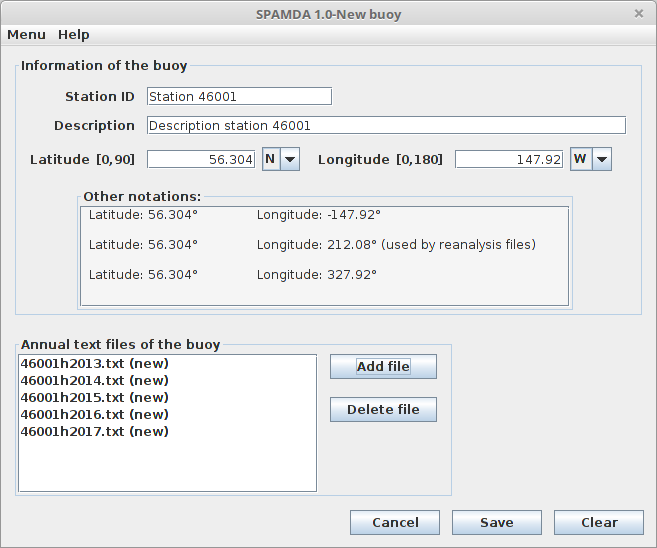
\includegraphics[scale=0.41]{figures/enteringBuoy.png}
					\caption{Entering a new buoy.}
					\label{fig:enteringBuoy}
				\end{figure}
				
				In the same way, by clicking on the \textcolor{blue}{\textit{View/Modify}} button it is possible to view or modify the data relating to the selected buoy. To delete a buoy click on the \textcolor{blue}{\textit{Delete}} button.
				
				\begin{center}
					\begin{warningbox}{Warning}{12cm}
						Deleting a buoy will remove all the data related to the buoy.
					\end{warningbox}
				\end{center}
				
			\subsection{Datasets}\label{sec:Datasets}
			
				%The \textit{Datasets} tab, which is represented in Fig. \ref{fig:tabDatasets}, allows the researchers to manage the intermediate datasets needed for their studies and relating to each buoy.
				
				The \textit{Datasets} tab, which is represented in Fig. \ref{fig:tabDatasets}, allows the researchers to manage the intermediate datasets of each buoy, which are the baseline for their studies.
				
				\begin{figure}[ht!]
					\centering
					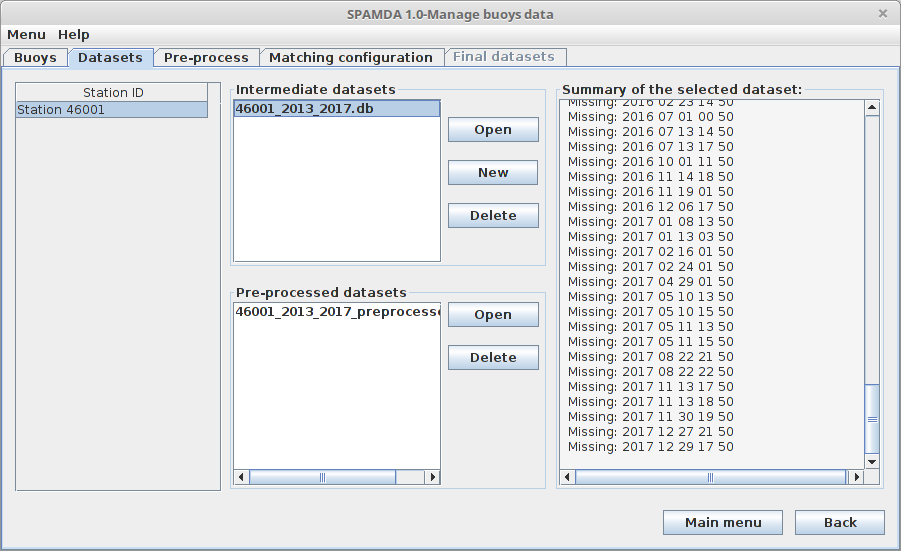
\includegraphics[scale=0.40]{figures/tabDatasets.png}
					\caption{Tab \textit{Datasets}.}
					\label{fig:tabDatasets}
				\end{figure}
			
				Once a buoy has been entered it is possible to create intermediate datasets using one ore more annual text files (added previously), which contain the measurements collected by the buoy. Note that such measurements may be incomplete or recorded at a different time than the expected one due to the weather conditions in which the buoys have to operate. SPAMDA has been designed to tackle such situation and it informs the researchers of any incidence found while reading the annual text files for creating the intermediate datasets.
				
				When an intermediate dataset is created, it is associated with its corresponding buoy, enabling the researchers to identify which intermediate datasets belong to each buoy. Besides, a summary of the content of the intermediate dataset is also created, providing relevant information about its content such as number of instances, date of first and last measurement, annual text files included, missing and duplicated dates.
				
				To proceed with the creation of an intermediate dataset follow the next steps:
				
					\begin{itemize}\itemsep0.02cm
						\item \textit{\textbf{Step 1}}: Select the desired buoy from the list shown on the left side.
						\item \textit{\textbf{Step 2}}: Click on the \textcolor{blue}{\textit{New}} button, then the view represented in Fig. \ref{fig:creatingIntermediateDataset} will be displayed. (The remaining steps are related to such view).
							\begin{figure}[ht!]
								\centering
								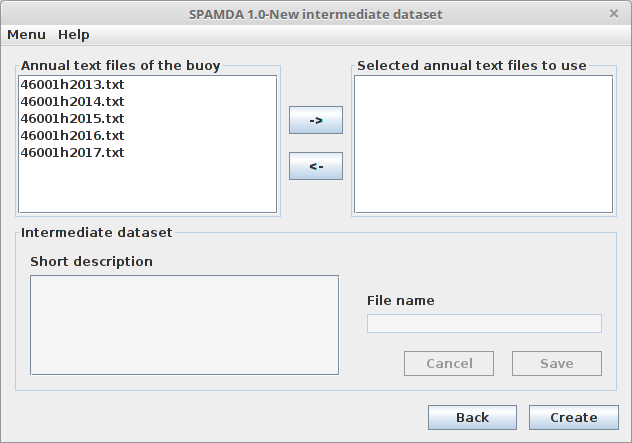
\includegraphics[scale=0.38]{figures/creatingIntermediateDataset.png}
								\caption{New intermediate dataset view.}
								\label{fig:creatingIntermediateDataset}
							\end{figure}
						\item \textit{\textbf{Step 3}}: Select the annual text files to use by clicking on the \textcolor{blue}{\textit{$-$$>$}} button. To deselect a previously selected file click on the \textcolor{blue}{\textit{$<$$-$}} button.
						\item \textit{\textbf{Step 4}}: When finished the selection click on the \textcolor{blue}{\textit{Create}} button.
						\item \textit{\textbf{Step 5}}: Type the description and the name of the intermediate dataset and click on the \textcolor{blue}{\textit{Save}} button to start the process of creation.
					\end{itemize}
					
				After that, SPAMDA will show the status of such process and the incidences that were found in the data, when it finished click on the \textcolor{blue}{\textit{Ok}} button. Note that the process can be cancelled by clicking on the \textcolor{blue}{\textit{Cancel creation}} button.
				
				The view that shows the status of the process of creation of an intermediate dataset for the buoy identified as \textit{Station 46001} using the annual text files of the years $2013$, $2014$, $2015$, $2016$ and $2017$ is represented in Fig. \ref{fig:statusCreationIntermediateDataset}.
			
					\begin{figure}[ht!]
						\centering
						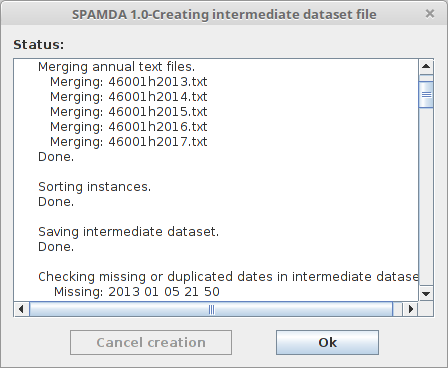
\includegraphics[scale=0.39]{figures/statusCreationIntermediateDataset.png}
						\caption{Status of the creation of the intermediate dataset.}
						\label{fig:statusCreationIntermediateDataset}
					\end{figure}
					
				%As it is shown in Fig. \ref{fig:tabDatasets} when a buoy is selected the intermediate datasets belonging to it are displayed, similarly occurs with the pre-processed datasets (which will be described in Section \ref{sec:Preprocess}) when selecting an intermediate dataset. Besides, on the right side is showed the summary of the intermediate or pre-processed dataset selected.
				
				As it is shown in Fig. \ref{fig:tabDatasets} when a buoy is selected, the intermediate datasets belonging to it are displayed, similarly, if one of these intermediate datasets  is selected, the pre-processed datasets (described in Section \ref{sec:Preprocess}) obtained from it are displayed. Besides, on the right side the summary of the intermediate or pre-processed dataset selected is shown.
				
				By clicking on the corresponding \textcolor{blue}{\textit{Delete}} button, the intermediate or pre-processed dataset selected will be removed.
				
				\begin{center}
					\begin{warningbox}{Warning}{13cm}
						Deleting an intermediate dataset will also remove all the pre-processed datasets belonging to it.
					\end{warningbox}
				\end{center}
				
				On the other hand, when clicking on the corresponding \textcolor{blue}{\textit{Open}} button the application will be redirected to the \textit{Pre-process} tab (see Section \ref{sec:Preprocess}) and the selected dataset (intermediate or pre-processed) will be opened for being pre-processed.
			
			\subsection{Pre-process}\label{sec:Preprocess}
			
				%The \textit{Preprocess} tab, which is represented in Fig. \ref{fig:tabPreprocess}, provides data pre-processing, which is useful for transforming raw data (intermediate datasets) into \textit{clean} and \textit{tidy} data. In this way, the quality of data can be improved prior to computational learning by ML techniques.
				
				The \textit{Pre-process} tab, which is represented in Fig. \ref{fig:tabPreprocess}, allows to perform data pre-processing, which prepares the raw data (intermediate datasets) to be able to be treated correctly by ML algorithms. In this way, the quality of data can be improved prior to computational learning.
				
				\begin{figure}[ht!]
					\centering
					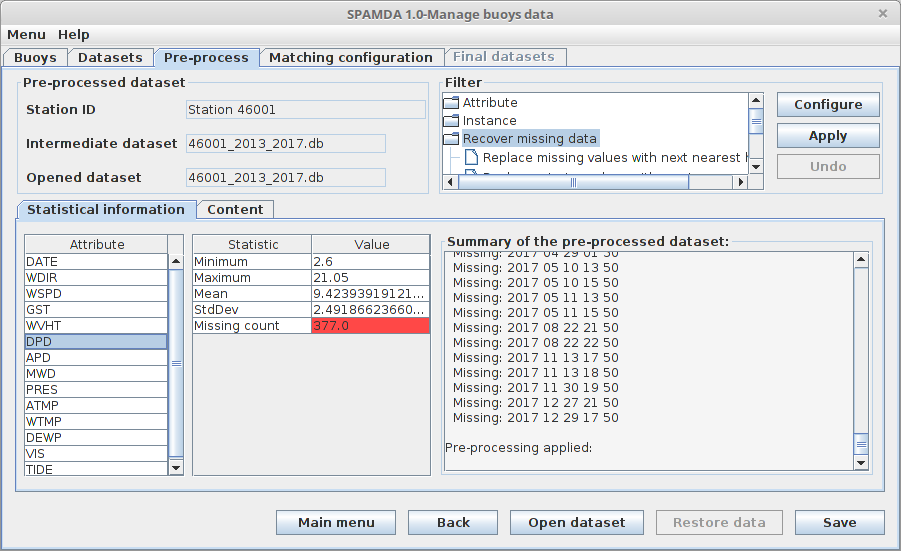
\includegraphics[scale=0.40]{figures/tabPreprocess.png}
					\caption{Tab \textit{Pre-process}.}
					\label{fig:tabPreprocess}
				\end{figure}
			
				Once an intermediate dataset has been created it is possible to apply the necessary pre-processing tasks (filters) to enhance the data quality. In the \textcolor{blue}{\textit{Statistical information}} tab relevant data about each attribute of the opened dataset (the one is currently being pre-processed) such as number of instances with missing values, minimum and maximum values, mean and standard deviation is shown. Providing the researchers the capacity to evaluate the pre-processing being performed.
				
				SPAMDA provides several configurable filters grouped in three categories, \textit{Attribute}, \textit{Instance} and \textit{Recover missing data}:
				
				\begin{itemize}
					\item \textit{Attribute}: All these filters can be applied to the attributes of the opened dataset.
						\begin{itemize}
							\item \textit{Normalize} \cite{WEKA_Filter_Normalize}: This filter normalises all numeric values of each attribute. The resulting values are by default in [0,1] for the data used to compute the normalisation intervals.
							\item \textit{Remove} \cite{WEKA_Filter_Remove}: It removes an attribute or a range of them.
							\item \textit{RemoveByName} \cite{WEKA_Filter_RemoveByName}: It allows to remove attributes based on a regular expression matched against their names.
							\item \textit{ReplaceMissingValues} \cite{WEKA_Filter_ReplaceMissingValues}: For each attribute all the missing values will be replaced with its mean.
							\item \textit{ReplaceMissingWithUserConstant} \cite{WEKA_Filter_ReplaceMissingWithUserConstant}: This filter replaces all the missing values of the attributes with an user-supplied constant value.
						\end{itemize}
				 \item \textit{Instance}: All these filters can be applied to the instances (hourly measurements) of the opened dataset.
					\begin{itemize}
						\item \textit{RemoveDuplicates} \cite{WEKA_Filter_RemoveDuplicates}: With this filter all duplicated instances are removed.
						\item \textit{RemoveWithValues} \cite{WEKA_Filter_RemoveWithValues}: This filter removes all the instances that match on the attribute and value user-supplied.
						\item \textit{SubsetByExpression} \cite{WEKA_Filter_SubsetByExpression}: It removes all the instances which don't match on a user-specified expression.
					\end{itemize}
				 \item \textit{Recover missing data}: All these filters can be applied to the instances of the opened dataset.
					\begin{itemize}
						\item \textit{Replace missing values with next nearest hour}: The missing values of each attribute are replaced with the next nearest non missing value.
						\item \textit{Replace missing values with previous nearest hour}: This filter replaces the missing values of each attribute with the previous nearest non missing value.
						\item \textit{Replace missing values with next $n$ hours mean}: The missing values of each attribute are replaced with the next $n$ nearest (configurable) non missing values mean. Note that these values may not coincide with the next $n$ hours.
						\item \textit{Replace missing values with previous $n$ hours mean}: This filter replaces the missing values of each attribute with the previous $n$ nearest non missing values mean. Note that these values may not coincide with the previous $n$ hours.
						\item \textit{Replace missing values with symmetric $n$ hours mean}: The missing values of each attribute are replaced with the $n$ previous and $n$ next non missing values mean. Note that these values may not coincide with the symmetric $n$ hours.
					\end{itemize}
				\end{itemize}
				
				%As a result of the data pre-processing it is possible to create new datasets, which are referenced as pre-processed datasets. Besides, a pre-processed dataset can be also pre-processed again enabling the researchers to resume such task at any other time.
				
				Once the pre-processing has been performed it is possible to save the resulting dataset, which will be referenced as a pre-processed dataset in SPAMDA. Besides, a pre-processed dataset can be also pre-processed again enabling the researchers to resume such task at any other time.
				
				To apply a filter follow the next steps:
				
					\begin{itemize}
						\item \textit{\textbf{Step 1}}: Open the desired intermediate or pre-processed dataset by clicking on either the \textcolor{blue}{\textit{Open dataset}} button or the corresponding \textcolor{blue}{\textit{Open}} button of tab \textit{Datasets}.
						\item \textit{\textbf{Step 2}}: Select one of the available filters.
						\item \textit{\textbf{Step 3}}: Configure the filter if necessary by clicking on the \textcolor{blue}{\textit{Configure}} button.
						\item \textit{\textbf{Step 4}}: Apply the filter by clicking on the \textcolor{blue}{\textit{Apply}} button.
					\end{itemize}
					
				As shown in Fig. \ref{fig:tabPreprocess} the pre-processing tasks performed on the opened dataset are displayed on the right side. SPAMDA allows the researchers to undo the last filter applied (\textcolor{blue}{\textit{Undo}} button) or to restore the initial content of the dataset (\textcolor{blue}{\textit{Restore data}} button).
				
				To create a pre-processed dataset follow the next steps:
				
					\begin{itemize}
						\item \textit{\textbf{Step 1}}: Click on the \textcolor{blue}{\textit{Save}} button, then the view represented in Fig. \ref{fig:creatingPreProcessedDataset} will be displayed. (The remaining step is related to such view).
							\begin{figure}[ht!]
								\centering
								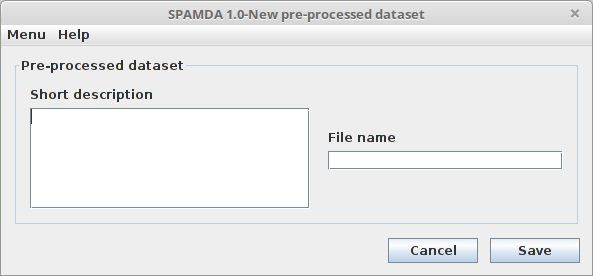
\includegraphics[scale=0.40]{figures/creatingPreProcessedDataset.png}
								\caption{New pre-processed dataset view.}
								\label{fig:creatingPreProcessedDataset}
							\end{figure}
						\item \textit{\textbf{Step 2}}: Type the description and the name of the pre-processed dataset and click on the \textcolor{blue}{\textit{Save}} button.
					\end{itemize}
					
				When saving the pre-processed dataset it will be associated with its corresponding intermediate dataset.

				Moreover, it is also possible to visualise the content of the opened dataset, enabling the researchers to easily identify if any of the instances is missing, duplicated, incomplete (missing values) or was recorded at a different time than the expected one, as mentioned in Section \ref{sec:Datasets}. To proceed with such action click on the \textcolor{blue}{\textit{Content}} tab and use the buttons \textcolor{blue}{\textit{$>$}} and \textcolor{blue}{\textit{$<$}} to check the possible affected instances as it is shown in Fig. \ref{fig:contentOpenedDataset}.
				
				\begin{figure}[ht!]
					\centering
					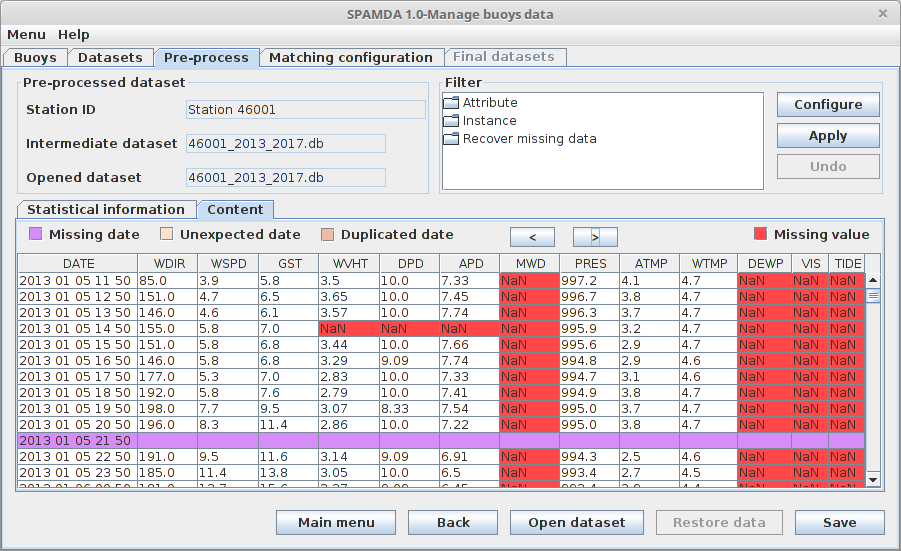
\includegraphics[scale=0.40]{figures/contentOpenedDataset.png}
					\caption{Visualising the content of the opened dataset.}
					\label{fig:contentOpenedDataset}
				\end{figure}
			
			\subsection{Matching configuration}\label{sec:MatchingConf}
			
				The \textit{Matching configuration} tab, which is represented in Fig. \ref{fig:tabMatchingConfiguration}, allows the researchers to customise the parameters of the matching process, which is necessary to carry out in order to merge and format the data provided by the two sources of information described in Section \ref{sec:DataSources}.
				
				\begin{figure}[ht!]
					\centering
					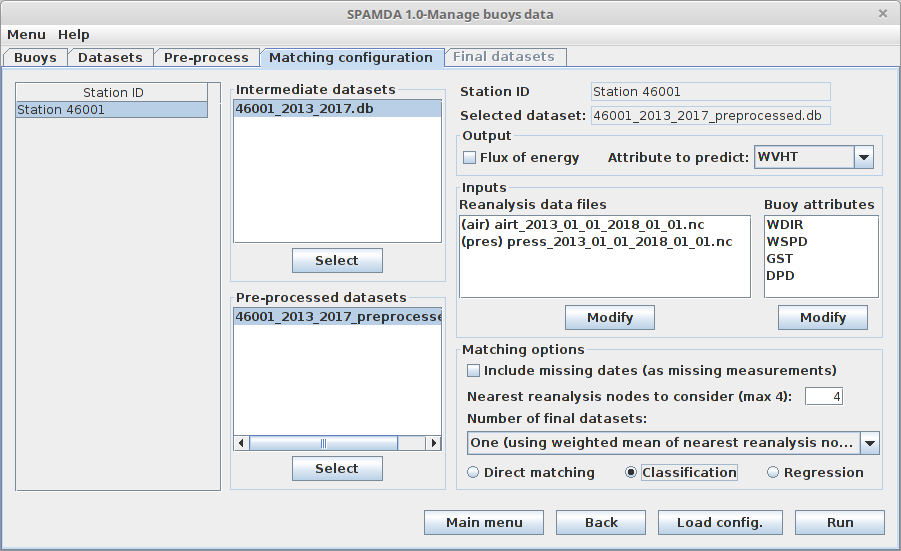
\includegraphics[scale=0.40]{figures/tabMatchingConfiguration.png}
					\caption{Tab \textit{Matching configuration}.}
					\label{fig:tabMatchingConfiguration}
				\end{figure}
			
				The matching procedure is performed using an intermediate or pre-processed dataset, which includes the measurements collected by a buoy from NDBC, and also the corresponding reanalysis data files from NNRP. Note that SPAMDA is able to manage the NetCDF binary format for handling the information stored in such reanalysis files.
				
				%Such process merges the information of both sources that matches on time, but due to that the measurements of the buoys are hourly collected from $00$:$50$ to $23$:$50$ UTC, and the reanalysis data is available every $6$ hours at $00$Z, $06$Z, $12$Z and $18$Z, the matching can only be carried out each $6$ hours (discarding the unused measurements from the buoy data). Besides, and since there is still a difference of 10 minutes, the matching with the reanalysis data will be performed with the nearest measurement (previous or next) within a maximum of 60 minutes of difference. Finally, the matched instances of both sources will result in the final datasets.
				
				Such process merges the information of both sources that match on time, but due to the measurements of the buoys are hourly collected from $00$:$50$ to $23$:$50$ UTC, and the reanalysis data is available every $6$ hours at $00$Z, $06$Z, $12$Z and $18$Z, the matching can only be carried out each $6$ hours (discarding the unused measurements from the buoy data). Besides, and since there is still a difference of 10 minutes, the matching with the reanalysis data will be performed with the nearest measurement (previous or next) within a maximum of 60 minutes of difference. Finally, the matched instances of both sources will result in the final datasets.
				
				SPAMDA allows the researchers to perform a customisable matching process, through which the researchers can easily obtain as different final datasets of the same meteorological data as needed, allowing them to consider different factors of the problem under study. These final datasets can be used for classification or regression prediction tasks, or direct matching. Prediction tasks are used to estimate the value of the output attribute in a concrete future using the information provided by the input attributes. Depending on the task to use, the final datasets must be prepared and configured in a specific way:
				
				\begin{itemize}
					\item \textit{Classification}: The final datasets will be ready to use as input in classification methods, which require a nominal output attribute and whose specific preparation is explained in Section \ref{sec:FinalDatasets}.
					\item \textit{Regression}: The final datasets will be ready to use as input in regression methods, which require a real output attribute and whose preparation is also explained in Section \ref{sec:FinalDatasets}.
					\item \textit{Direct matching}: In this case the inputs attributes have a direct correspondence with the output attribute, and it is not necessary to perform any additional preparation. For example, the final datasets may be used in lost data recovering tasks, or in the way the researchers consider suitable according to the problem under study.
				\end{itemize}
				
				Following, the parameters that can be configured in the matching process are described:
				
				\begin{itemize}
				
					\item \textit{Flux of energy} \cite{FERNANDEZ201544}: When the $F_e$ is selected, it will be used as output. This attribute is not collected by the buoys, but it can be calculated from two wave parameters: $H_s$ and $T_e$, which are collected as WVHT and APD attributes respectively. In this way, SPAMDA will obtain the $F_e$ of each instance using the following equation:
					
						\begin{equation}
							F_e = 0.49 \cdot H^2_s \cdot T_e
							\label{eq:fluxOfEnergy}
						\end{equation}
					
					where $F_e$ is measured in kilowatts per meter, $H_s$ is measured in meters and $T_e$ is measured in seconds. Note also that $F_e$ is defined in Eq. \ref{eq:fluxOfEnergy} as an average energy flux ($H_s$ is a kind of average wave height), though for simplicity it will be referred just as flux of energy.
					
					\item \textit{Attribute to predict}: Instead of using the $F_e$, the researchers can select any of the attributes collected by the buoys as output (e.g. significant wave height (WVHT), wind direction (WDIR), sea level pressure (PRES), etc.). Therefore, they can focus on different studies by selecting an attribute or other.

					\item \textit{Reanalysis data files}: In order to have a more accurate description of the problem under study, more than one reanalysis variable can be considered as input. Remember that these files have to be previously downloaded by the researcher from the website of the NNRP \cite{NNRP}, which should set the range of dates (temporal properties) and the desired sub-grid (spatial properties, see Fig. \ref{fig:subGrid}) for each variable of reanalysis. In that sense, the reanalysis data files must have the same spatial and temporal properties but relating to different variables each other.
					
					To select the needed reanalysis data files click on the corresponding \textcolor{blue}{\textit{Add/Modify}} button and the view represented in Fig. \ref{fig:selectingReanalysisDataFiles} will be displayed. SPAMDA facilitates this task by showing in cyan colour the reanalysis data files that are compatibles each other when selecting or clicking on a file. Click on the \textcolor{blue}{\textit{Confirm selection}} button when finished and SPAMDA will check that the selected files meet such condition.
					
					\begin{figure}[ht!]
						\centering
						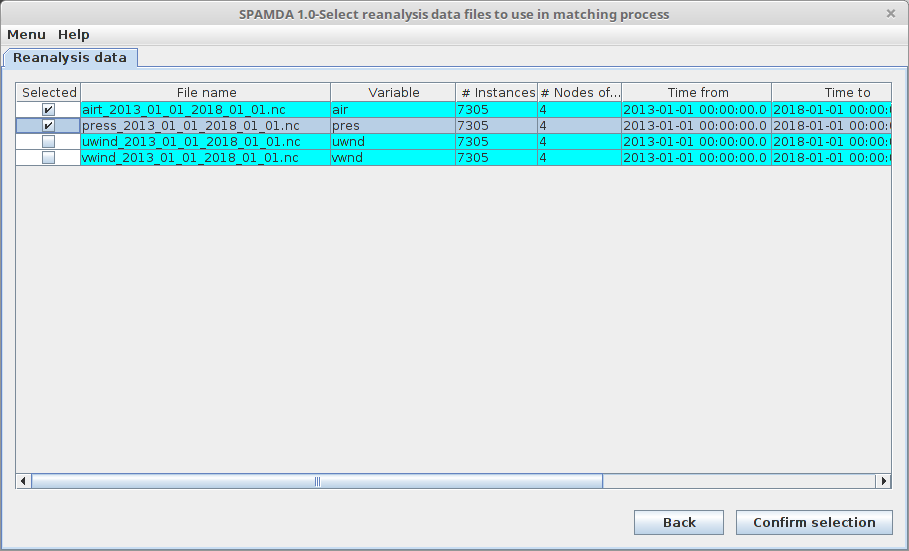
\includegraphics[scale=0.40]{figures/selectingReanalysisDataFiles.png}
						\caption{Selecting reanalysis data files.}
						\label{fig:selectingReanalysisDataFiles}
					\end{figure}

					\item \textit{Buoys attributes}: In addition to the reanalysis variables, the final datasets will also include the selected attributes as inputs (of the intermediate or pre-processed dataset used), providing a possible better characterisation of the problem under study, although it will depend on how correlated the attributes are.
					
					In the same way, in order to select the attributes of the buoy click on the corresponding \textcolor{blue}{\textit{Add/Modify}} button and the view represented in Fig. \ref{fig:selectingBuoysAttributes} will be displayed showing the available attributes of the buoy.
					
					\begin{figure}[ht!]
						\centering
						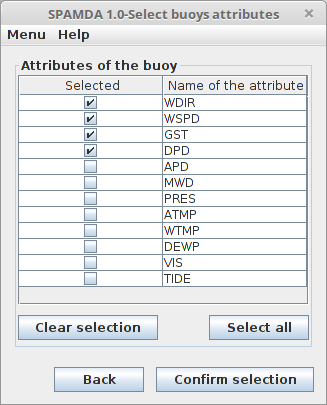
\includegraphics[scale=0.40]{figures/selectingBuoysAttributes.png}
						\caption{Selecting buoys attributes.}
						\label{fig:selectingBuoysAttributes}
					\end{figure}
					
					Once done the selection click on the \textcolor{blue}{\textit{Confirm selection}} button.
					
					\item \textit{Include missing dates}: As mentioned in Section \ref{sec:Datasets}, the information collected by a buoy may be incomplete due to measurements not recorded by it. As a consequence, the matching of instances between both sources of information may mismatch (missing dates). In that situation, the researchers can consider two options: 1) discard the instances affected or 2) include them. In the latter case, the final datasets will contain the affected instances, but the measurements of the buoy will be stored as missing values in WEKA format, denoted as \guillemotleft\textit{?}\guillemotright.
					
					\item \textit{Nearest reanalysis nodes to consider}: As already shown in Fig. \ref{fig:subGrid}, the reanalysis data files may contain information of several reanalysis nodes. In this way, this parameter allows the researchers to choose from:
					
						\begin{itemize}
						
							\item Consider all the reanalysis nodes: in this case, all the information of each selected reanalysis data file will be used.
							
							\item Consider only some of the reanalysis nodes: in this case, only the information of the $N$ closets reanalysis nodes (configurable) to the buoy will be used. To do that, SPAMDA uses the \textit{Haversine} formula \cite{Haversine_2009} to calculate the distance from each reanalysis node to the localisation of the buoy and obtain the closest ones. Haversine formula is also known as great circle distance, this formula perform calculation from main point to destination point with trigonometric function by using latitude and longitude. Haversine formula is calculated as follows:
							  \begin{linenomath*}
									\begin{equation}
										d(p_0,p_j)=\arccos(\sin(lat_0)\cdot \sin(lat_j)\cdot \cos(lon_0-lon_j) + \cos(lat_0) \cdot \cos(lat_j)),
										\label{eq:Haversine}
									\end{equation}
								\end{linenomath*}
							where $p_0$ is the buoy geographical localisation, $p_j$ stands for the location of each reanalysis node, and $lat$ and $lon$ are the latitude and longitude of the points, respectively.
							
						\end{itemize}
					
					\item \textit{Number of final datasets}: Depending on the number of the nearest reanalysis nodes to consider, the number of the final datasets to create and therefore the content of them can be configured according to the following options:

						\begin{itemize}
							%\item \textit{One (using weighted mean of $N$ nearest reanalysis nodes)}: Only one final dataset will be created, which will contain the attributes (the selected one as output and the selected ones as inputs) of the intermediate or pre-processed dataset used, along with a weighted mean of each variable of reanalysis used (one per selected reanalysis data file). This weighted mean takes into account the distance from each reanalysis node to the localisation of the buoy, and it is calculated by SPAMDA using the formula defined in Eq. \ref{eq:weightedMean}. Therefore, the closest reanalysis nodes to the localisation of the buoy will provide more information.
							
							\item \textit{One (using weighted mean of $N$ nearest reanalysis nodes)}: Only one final dataset will be created, which will contain the attributes (the selected one as output and the selected ones as inputs) of the intermediate or pre-processed dataset used, along with a weighted mean of each variable of reanalysis used (one per selected reanalysis data file). This weighted mean is obtained by SPAMDA and uses the distance (using the formula defined in Eq. \ref{eq:Haversine}) from each reanalysis node to the localisation of the buoy. Once the distances have been calculated they are inverted and normalised as follows:
							
								\begin{linenomath*}
									\begin{equation}
										w_i=\frac{\sum_{j=1}^{N} d(p_0,p_j)}{d(p_0,p_i)}, ~~i=1, \ldots, N.
										\label{eq:weightedMean}
									\end{equation}
								\end{linenomath*}
							
							After calculating these weights, they are applied to obtain a weighted mean of each variable of reanalysis. Therefore, the closest reanalysis nodes to the localisation of the buoy will provide more information.
							
							Considering as example the two nearest reanalysis nodes represented in Fig. \ref{fig:subGrid} and the reanalysis variables air temperature and pressure, the weighted mean of each reanalysis variable will be calculated using the reanalysis nodes $57.5$ N $\times$ $147.5$ W and $55.0$ N $\times$ $147.5$ W.
							
							\item \textit{'N' (one per each reanalysis node)}: As many final datasets as number of nearest $N$ reanalysis nodes configured by the researcher will be created. Therefore, each final dataset will contain the value of each reanalysis variable used of the nearest corresponding reanalysis node, along with the selected attributes of the intermediate or pre-processed dataset used.
							
							In this case, and considering as example the four closest reanalysis nodes (see Fig. \ref{fig:subGrid}) and the reanalysis variables air temperature and pressure, then only four final datasets will be created, containing each one the information of both reanalysis variables of the corresponding reanalysis node: $57.5$ N $\times$ $147.5$ W, $55.0$ N $\times$ $147.5$ W, $57.5$ N $\times$ $150.0$ W and $55.0$ N $\times$ $150.0$ W, along with the selected attributes of the intermediate or pre-processed dataset used.
							
						\end{itemize}
						
				\end{itemize}
				
				To proceed with the matching process follow the next steps:
				
					\begin{itemize}
						\item \textit{\textbf{Step 1}}: Select the desired buoy from the shown on the left side.
						\item \textit{\textbf{Step 2}}: Select the intermediate or pre-processed dataset to use.
						\item \textit{\textbf{Step 3}}: Configure the above-mentioned matching parameters and click on the \textcolor{blue}{\textit{Run}} button to start the matching process.
					\end{itemize}
					
				Then, SPAMDA will show the status of such process and the missing dates that were found, when it finished click on the \textcolor{blue}{\textit{OK}} button and the application will be redirected to the \textit{Final datasets} tab (see Section \ref{sec:FinalDatasets}) to perform the preparation of the matched data.
				
				In Fig. \ref{fig:statusMatchingProcess} is represented the status of a matching process using the configuration showed in Fig. \ref{fig:tabMatchingConfiguration}.
				
					\begin{figure}[ht!]
						\centering
						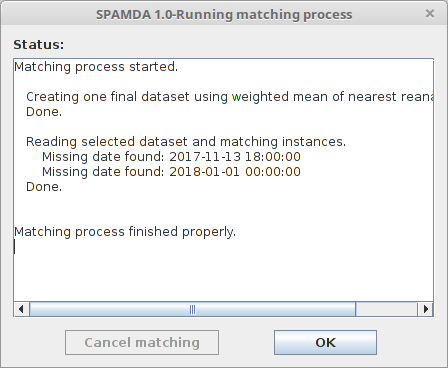
\includegraphics[scale=0.40]{figures/statusMatchingProcess.png}
						\caption{Status of the matching process.}
						\label{fig:statusMatchingProcess}
					\end{figure}
				
				Instead of typing all the required parameters, it is possible to load a previously matching configuration saved. To do that click on the \textcolor{blue}{\textit{Load config.}} button, then the view represented in Fig. \ref{fig:selectingMatchingConfiguration} will be displayed for selecting the configuration to be loaded (Section \ref{sec:FinalDatasets} describes how to save the configuration used in the matching process and for the preparation of the matched data).
				
				\begin{figure}[ht!]
					\centering
					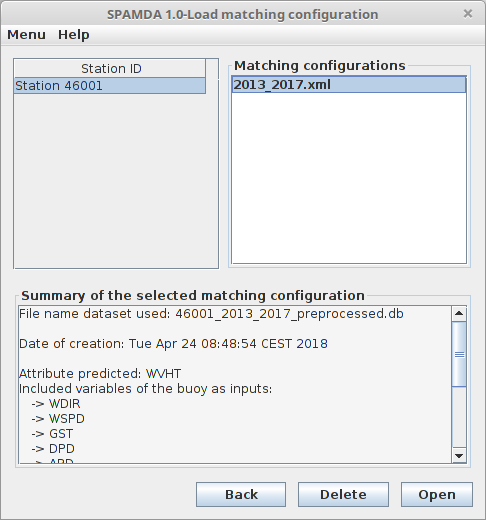
\includegraphics[scale=0.40]{figures/selectingMatchingConfiguration.png}
					\caption{Load matching configuration.}
					\label{fig:selectingMatchingConfiguration}
				\end{figure}
				

			\subsection{Final datasets}\label{sec:FinalDatasets}
			
				The \textit{Final datasets} tab, which is represented in Fig. \ref{fig:tabFinalDatasets}, permits the researchers to prepare the matched data for the desired prediction task (\textit{Regression} or \textit{Classification}), obtaining as a result the final datasets. Remember that \textit{Direct matching}, as it was described in Section \ref{sec:MatchingConf}, performs a direct correspondence between the attributes used as inputs and the output one, and it is not necessary to carry out any preparation.
				
				\begin{figure}[ht!]
					\centering
					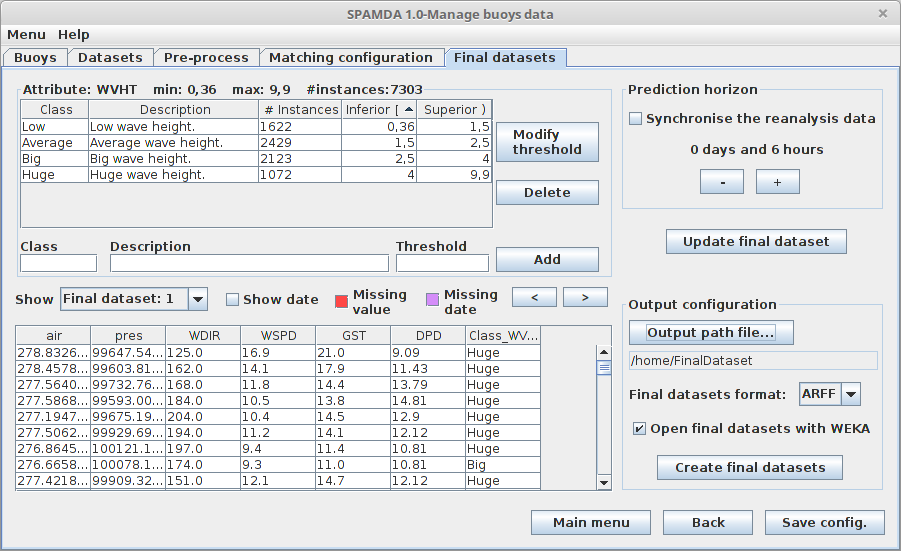
\includegraphics[scale=0.40]{figures/tabFinalDatasets.png}
					\caption{Tab \textit{Final datasets}.}
					\label{fig:tabFinalDatasets}
				\end{figure}
				
				SPAMDA allows the researchers to make such preparation by means of the following options:
				
					\begin{itemize}
						\item \textit{Prediction horizon} (Classification and Regression): This option indicates the time gap for moving backward the output attribute. In this way, the input attributes (variables of the buoy and reanalysis data) will be used to predict the output attribute in a concrete future (e.g. 6h, 12h, 18h, 1 day, etc.).
						
						The minimum interval for increasing and decreasing the prediction horizon is $6$h (due to reanalysis data temporal resolution) \cite{DORADOMORENO2017428}, the same interval used when the matching process is carried out. Therefore, for each increment of the prediction horizon an instance is lost from the end of the final datasets. As the minimum prediction horizon is $6$h at least one instance will be lost. The relation between the inputs and the attribute to predict will be defined as follows:
						
						\begin{linenomath*}
								\begin{equation}
									o_{t+\Delta t}=\phi(\mathbf{b}_t,\mathbf{r}_{t})
								\end{equation}
							\end{linenomath*}
						
						Where $t$ represents the time instant to study and $\Delta t$ the prediction horizon; $o$ is the attribute to predict, $\mathbf{b}$ is the vector containing the selected NDBC variables and $\mathbf{r}$ is the vector containing the selected reanalysis variables. Optionally, the reanalysis variables can be synchronised with the attribute to predict. Given that such variables are estimated by a mathematical model, it is allowed to use these future values, which could improve the performance of the results. In this case, the relation between the inputs and the attribute to predict would be:
						
							\begin{linenomath*}
								\begin{equation}
									o_{t+\Delta t}=\phi(\mathbf{b}_t,\mathbf{r}_{t+\Delta t})
								\end{equation}
							\end{linenomath*}
						
						\item \textit{Thresholds of the output attribute} (Classification): Since the values of the variables collected by the buoys are real numbers, it is necessary to discretise (convert from real to nominal values) the selected attribute as output. SPAMDA allows the researchers to perform this process by defining the necessary classes with their thresholds, which will be used against the values of the output attribute to carry out such discretisation.
					\end{itemize}
					
				Follow these steps to proceed with the preparation of the final datasets:
				
%					\begin{itemize}
%						\item \textit{\textbf{Step 1}}: Define the classes and its thresholds (\textit{Classification}).
%						\item \textit{\textbf{Step 2}}: Define the prediction horizon (\textit{Classification and Regression}).
%						\item \textit{\textbf{Step 3}}: Click on \textcolor{blue}{\textit{Update final dataset}} button.
%					\end{itemize}

					\begin{itemize}
						\item \textit{\textbf{Step 1}}: Define the classes and their thresholds (\textit{Classification}).
							\begin{itemize}
								\item To do that, use the buttons \textcolor{blue}{\textit{Add}}, \textcolor{blue}{\textit{Modify threshold}} or \textcolor{blue}{\textit{Delete}} to add a new threshold, modify or delete the selected one respectively.
							\end{itemize}
						\item \textit{\textbf{Step 2}}: Define the prediction horizon (\textit{Classification and Regression}).
							\begin{itemize}
								\item To do that, use the buttons \textcolor{blue}{\textit{$-$}} or \textcolor{blue}{\textit{$+$}} to decrease or increase the prediction horizon, and select or deselect the option \textcolor{blue}{\textit{Synchronise the reanalysis data}} depending on needs.
							\end{itemize}
						\item \textit{\textbf{Step 3}}: Click on the \textcolor{blue}{\textit{Update final dataset}} button to take the new configuration of the preparation.
					\end{itemize}
					
				Such preparation can be performed as many times as required and considering the typed options in each moment.
					
				As shown in Fig. \ref{fig:tabFinalDatasets}, the content of the final datasets obtained as a result of the custom preparation of the matched data, can be visualised enabling the researchers to check the final datasets before saving them on disk. Although the date will not be included in the final datasets, by selecting the \textcolor{blue}{\textit{Show date}} option it can be shown in order to know the dates of each instance of the intermediate or pre-processed dataset used, that matched with the reanalysis data. Moreover, by clicking on the \textcolor{blue}{\textit{$>$}} and \textcolor{blue}{\textit{$<$}} buttons it is possible to check the dates that were mismatched.

				Finally, and before creating the final datasets, it is necessary to define the output configuration:
			
				\begin{itemize}

					\item \textit{Output file}: Name of the final datasets and folder to save them on disk.
						
					\item \textit{Final datasets format}:

						\begin{itemize}
						
							\item \textit{ARFF}: \textit{Attribute-Relation File Format} \cite{WEKA_ARFF} which is used by the tool WEKA. SPAMDA allows the researchers to open the final datasets created with this format by running the environment Explorer of WEKA (in the same context of work), enabling they to choose the most appropriate ML method to tackle the problem under study. To do that select the option \textcolor{blue}{\textit{Open final datasets with WEKA}}.

							\item \textit{CSV}: \textit{Comma-Separated Values}. With this format the researchers may use the final datasets in the way they deem suitable.
							
						\end{itemize}
					
				\end{itemize}
				
				Once finished the preparation, by clicking on the \textcolor{blue}{\textit{Create final datasets}} button the final datasets will be saved on disk in the selected folder, an them will be opened by the tool WEKA, as represented in Fig. \ref{fig:openigFinalDatasetWeka}, if the researchers selected such option.
				
				\begin{figure}[ht!]
					\centering
					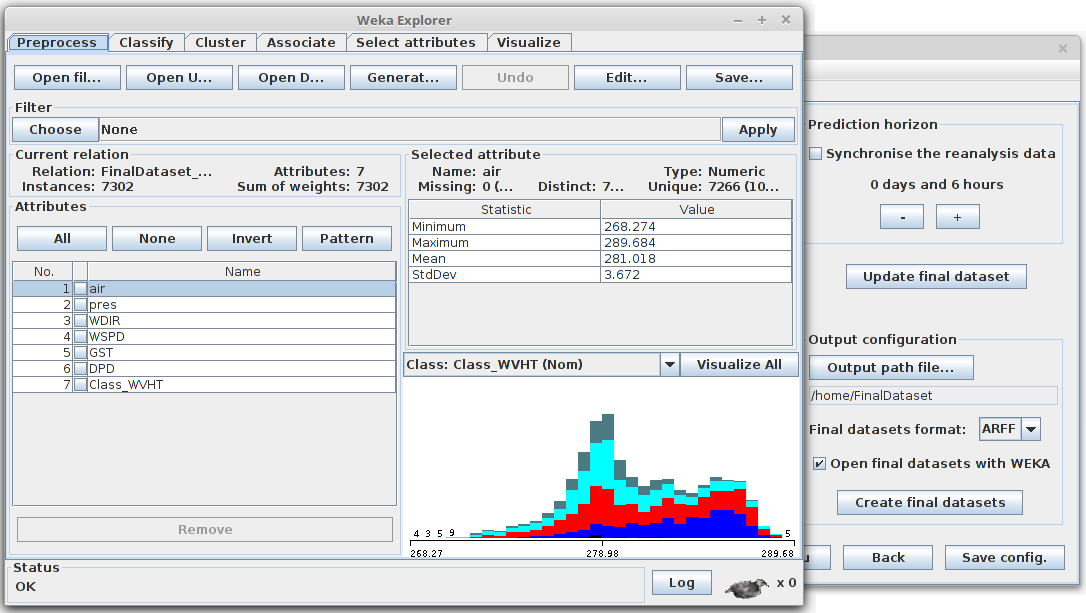
\includegraphics[scale=0.375]{figures/openigFinalDatasetWeka.png}
					\caption{Opening with WEKA the final dataset created.}
					\label{fig:openigFinalDatasetWeka}
				\end{figure}
				
				%Besides, a text file that summarises the configuration used in the matching process and for the preparation of the matched data is also generated in addition to the final datasets. 
				
				SPAMDA allows the researchers to save the configuration used in the matching process and for the preparation of the matched data, enabling the researchers to resume their studies at any other time. To do that click on the \textcolor{blue}{\textit{Save config.}} button, then the view represented in Fig. \ref{fig:creatingMatchingConfiguration} will be displayed. After typing the description and the file name click on the \textcolor{blue}{\textit{Save}} button to save the configuration, which will be associated with the buoy used.
				
				\begin{figure}[ht!]
					\centering
					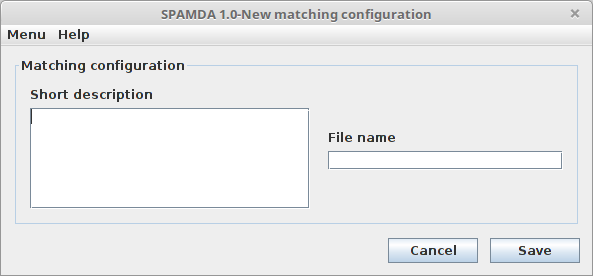
\includegraphics[scale=0.40]{figures/creatingMatchingConfiguration.png}
					\caption{New matching configuration.}
					\label{fig:creatingMatchingConfiguration}
				\end{figure}

		\section{Manage reanalysis data}
		
			This module, which is represented in Fig. \ref{fig:manageReanalysisData}, allows the management of the reanalysis data provided by NNRP. In this way, the researchers can keep up to date the reanalysis files needed for their studies. Remember that such data is available in NNRP web page \cite{NNRP}.
				\begin{figure}[ht!]
					\centering
					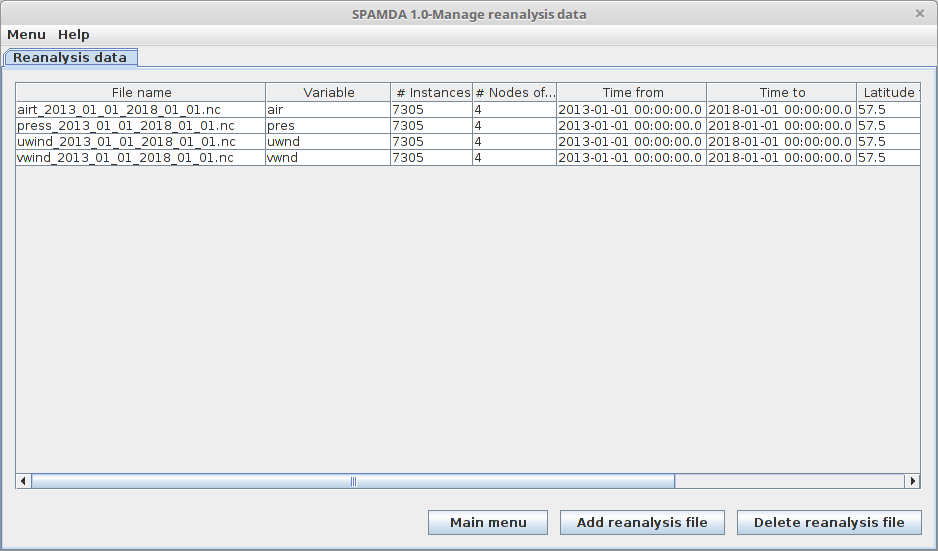
\includegraphics[scale=0.40]{figures/manageReanalysisData.png}
					\caption{Module Manage reanalysis data.}
					\label{fig:manageReanalysisData}
				\end{figure}
			
			To enter a new reanalysis file just click on the \textcolor{blue}{\textit{Add reanalysis file}} button and select the desired file, in order to delete a reanalysis file just click on the \textcolor{blue}{\textit{Delete reanalysis file}} button.
			
			As it is shown in Fig. \ref{fig:manageReanalysisData} useful information about the content of each reanalysis file can be consulted such as name of the file and the reanalysis variable, number of instances and reanalysis nodes, initial and final: time, latitude and longitude; which summarises the temporal and spatial properties of the data. Thus the researcher can quickly and easily identify each reanalysis file entered in SPAMDA.
		
		\section{Tools}
		
			This module includes two utilities, one for converting intermediate or pre-processed datasets to ARFF or CSV format and the other one for opening ARFF files with WEKA. Both features are accessible through the \textcolor{blue}{\textit{Tools}} option of the menu bar showed in Fig. \ref{fig:mainView}.
			
			\subsection{Datasets converter}
			
				This utility permits the researchers to convert the desired intermediate or pre-processed datasets to ARFF and CSV format. In this way, the researchers can use these converted datasets as they consider opportune.
				
				To convert an intermediate or pre-processed dataset click on the \textcolor{blue}{\textit{Dataset converter}} option and the view represented in Fig. \ref{fig:convertDatasets} will be displayed. On the left side are shown the buoys entered in SPAMDA, by clicking on one of them its intermediate datasets will be shown on the top side. Similarly, by clicking on one intermediate dataset its pre-processed datasets will be shown on the bottom side. Once selected the desired dataset (intermediate or pre-processed) just click on the \textcolor{blue}{\textit{Convert to ARFF}} or \textcolor{blue}{\textit{Convert to CSV}} button, and a dialog box will appear asking for the name of the target file that will be created as a result of the conversion.
				
					\begin{figure}[ht!]
						\centering
						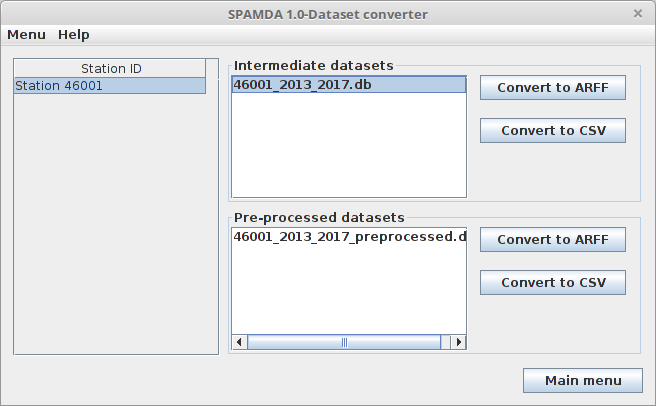
\includegraphics[scale=0.40]{figures/convertDatasets.png}
						\caption{Utility Dataset converter.}
						\label{fig:convertDatasets}
					\end{figure}
			
			\subsection{Open ARFF file with WEKA}
			
				This other utility allows the researchers to open ARFF files by running the environment Explorer of WEKA in the same context of work, enabling they to resume experiments with previously created final datasets.
				
				To open an ARFF file click on the \textcolor{blue}{\textit{Open ARFF file with WEKA}} option and the view represented in Fig. \ref{fig:openARFFfile} will be displayed.
				
					\begin{figure}[ht!]
						\centering
						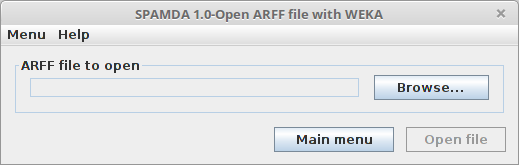
\includegraphics[scale=0.50]{figures/openARFFfile.png}
						\caption{Utility Open ARFF file with WEKA.}
						\label{fig:openARFFfile}
					\end{figure}
				
				To search for and select an ARFF file click on the \textcolor{blue}{\textit{Browse...}} button, when finished click on the \textcolor{blue}{\textit{Open file}} button for opening it and the view represented in Fig. \ref{fig:openingARFFFileWEKA} will be displayed.
					
					\begin{figure}[ht!]
						\centering
						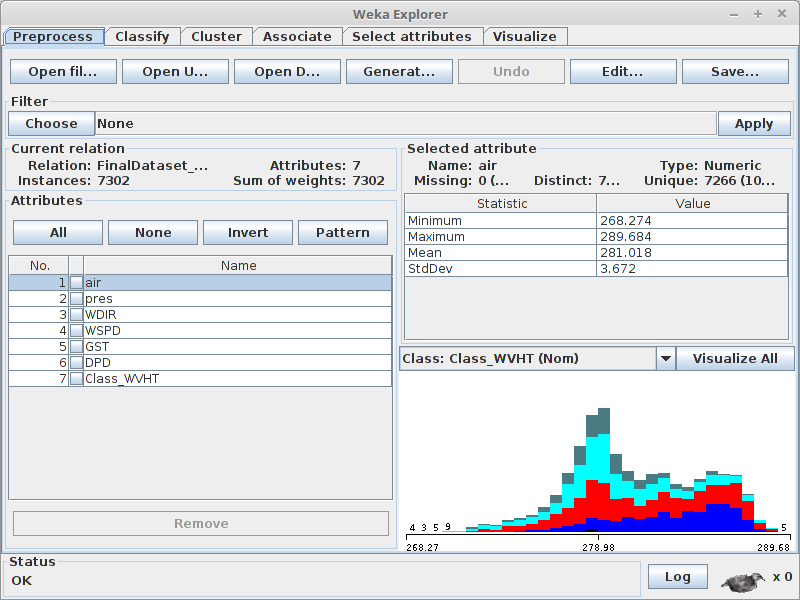
\includegraphics[scale=0.50]{figures/openingARFFFileWEKA.png}
						\caption{Opening an ARFF file with WEKA.}
						\label{fig:openingARFFFileWEKA}
					\end{figure}
					
				Remember that it is also possible to open the final datasets when creating them by selecting the option \textcolor{blue}{\textit{Open final datasets with WEKA}} (see Fig. \ref{fig:tabFinalDatasets}).
				
	\end{onehalfspace}

	
\chapter{Case study}

	\begin{onehalfspace}
	
		This chapter will describe how the application works in a practical approach. To do so, an example showing how to create a fully processed (final) dataset starting from the raw data will be performed. The objective of this final dataset is to be used in ML algorithms to classify waves in the Gulf of Alaska depending on their height.
		
		\section{Case study}
		
		The meteorological data that will be used to perform this case study is described bellow:
		
			\begin{enumerate}
			\item The measurements obtained from 2013 to 2017 by the buoy (46001) placed in the Gulf of Alaska, which are provided by NDBC as annual text files. This data is publicly available at the NDBC website. 
			\item Complementary information collected from reanalysis data containing air temperature, pressure and two components of wind speed (South-North and West-East) measurements. This information will be collected from the four closest reanalysis nodes surrounding the geographical location of the buoy. This data is publicly available at the NNRP website and can be downloaded in NetCDF format.
			\end{enumerate}

			After gathering the information described above \footnote{Further instructions for downloading this data can be found in Appendix \ref{app:GettingMetData}.}, the researcher can open SPAMDA.
			
			In Figure \ref{fig:main_view} the main view can be found, in order to input the reanalysis data which will be used in further steps for creating the final dataset, the researcher will select the option \textcolor{blue}{\textit{Manage reanalysis data}} from the view.
			
			\begin{figure}[ht]
				\centering
				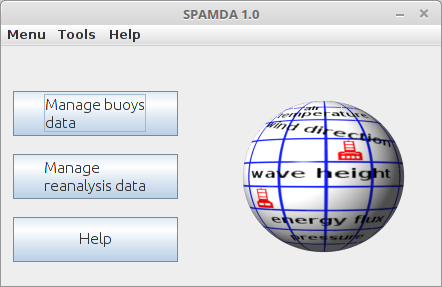
\includegraphics[scale=0.48]{figures/mainView.png}
				\caption{SPAMDA main view.}\label{fig:main_view}
			\end{figure}

			Then, the view represented in Figure \ref{fig:reanalysis} will appear. To enter the four reanalysis files (one per reanalysis variable) the researcher must click on the \textcolor{blue}{\textit{Add reanalysis file}} and a dialog box will appear for selecting them.
			
			\begin{figure}[ht!]
				\centering
				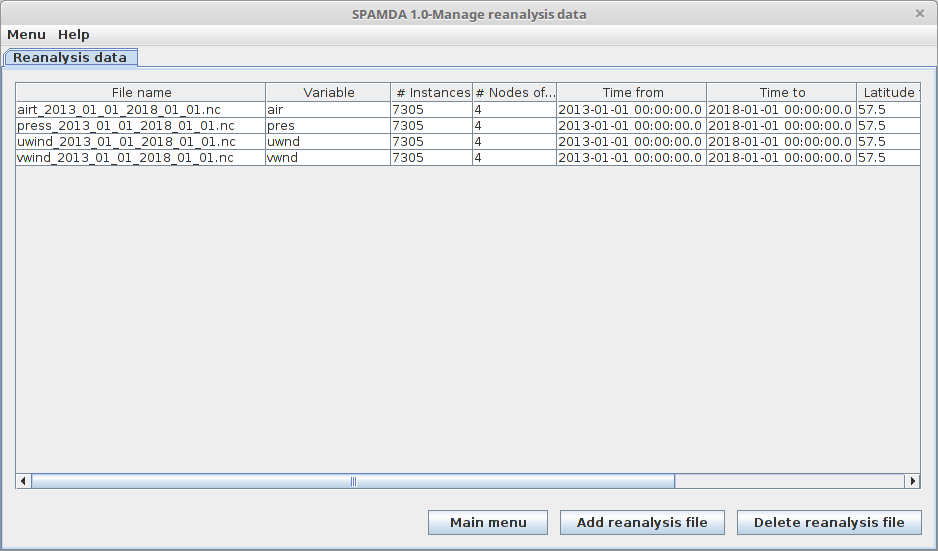
\includegraphics[scale=0.40]{figures/manageReanalysisData_CS.png}
				\caption{Module Manage reanalysis data.}\label{fig:reanalysis}
			\end{figure}
			
			After the reanalysis files has been introduced in SPAMDA, this window can be closed and go back to the main view to continue entering the information related to the buoy under study. The researcher will now select \textcolor{blue}{\textit{Manage buoys data}} to open the view shown in Figure \ref{fig:manage_buoys}. In order to enter such data, click on the \textcolor{blue}{\textit{New}} button, then the window shown in Figure \ref{fig:entering_buoy} will pop-up.
			
			\begin{figure}[ht!]
				\centering
				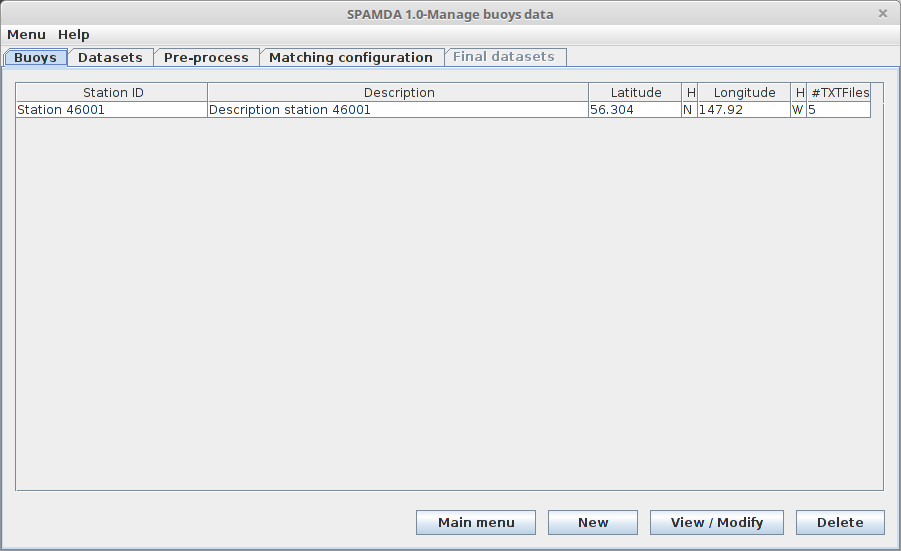
\includegraphics[scale=0.40]{figures/tabBuoys_CS.png}
				\caption{Tab \textit{Buoys}.}\label{fig:manage_buoys}
			\end{figure}

			\begin{figure}[ht!]
				\centering
				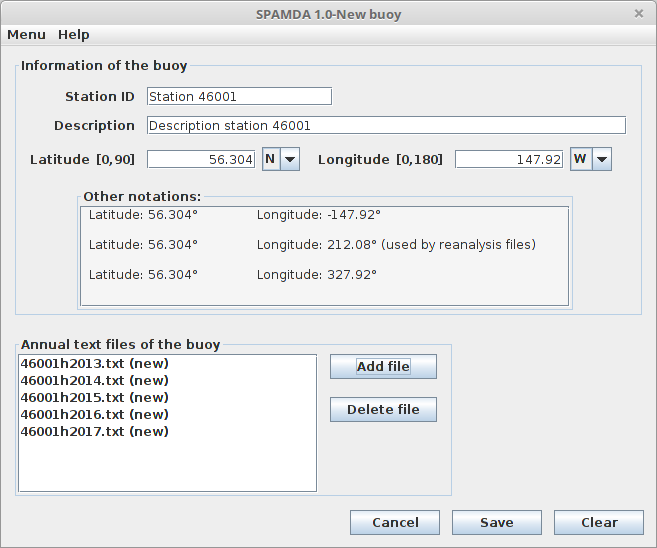
\includegraphics[scale=0.40]{figures/enteringBuoy_CS.png}
				\caption{Entering a new buoy.}\label{fig:entering_buoy}
			\end{figure}

			%Here the information about the buoy will be entered: the \textit{Station ID}, its description, geographical localisation and the corresponding annual text files. In this case, the files containing the data from year $2013$ to $2017$ are inserted. To do so, click on \textcolor{blue}{\textit{Add file}} button and a dialog box will appear for selecting them. Once the data has been introduced, it is necessary to click on \textcolor{blue}{\textit{Save}} button to insert the buoy in SPAMDA database, after that, the window can be closed. To proceed with the creation of the intermediate dataset, double-click on the buoy under study or click on the \textcolor{blue}{\textit{Datasets}} tab to switch to the next view (see Figure \ref{fig:show_datasets}).
			
			Here the information about the buoy will be entered: the \textit{Station ID}, its description, geographical localisation and the corresponding annual text files. In this case, the files containing the data from year $2013$ to $2017$ are inserted. To do so, click on the \textcolor{blue}{\textit{Add file}} button and a dialog box will appear for selecting them. Once the data has been introduced, it is necessary to click on the \textcolor{blue}{\textit{Save}} button to insert the buoy in SPAMDA database, after that, the window can be closed.

			\begin{figure}[ht!]
				\centering
				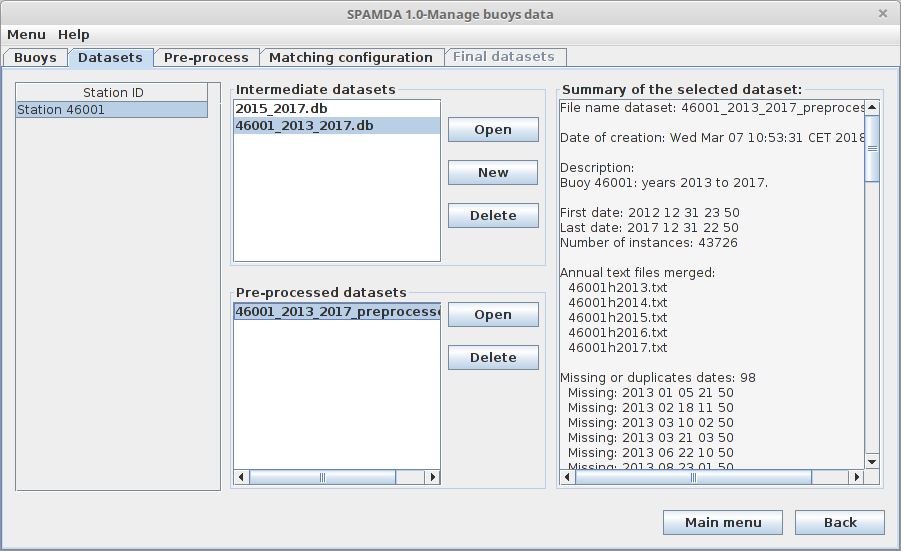
\includegraphics[scale=0.47]{figures/tabDatasets_CS.png}
				\caption{Tab \textit{Datasets}.}\label{fig:show_datasets}
			\end{figure}
			
			%The next step would be to create an intermediate dataset, the researcher will double-click on the buoy under study or click on the \textcolor{blue}{\textit{Datasets}} tab to switch to the next view (see Figure \ref{fig:show_datasets}). In this view, the researcher can delete or consult a brief of each intermediate or pre-processed dataset by selecting it from the corresponding list and also create new ones. To proceed with the creation of the intermediate dataset, click on the \textcolor{blue}{\textit{New}} button and the view shown in Figure \ref{fig:intermediate} will appear.
			
			The next step would be to create an intermediate dataset, the researcher will double-click on the buoy under study or click on the \textcolor{blue}{\textit{Datasets}} tab to switch to the next view (see Figure \ref{fig:show_datasets}).
			
			To proceed with the creation of the intermediate dataset, click on the \textcolor{blue}{\textit{New}} button and the view shown in Figure \ref{fig:intermediate} will appear. 
			
			%The next step would be to create an intermediate dataset including the desired annual text files of the buy. To do so, the researcher can click on \textcolor{blue}{\textit{New}} button and the view shown in Figure \ref{fig:intermediate} will appear.
			
			\begin{figure}[ht!]
				\centering
				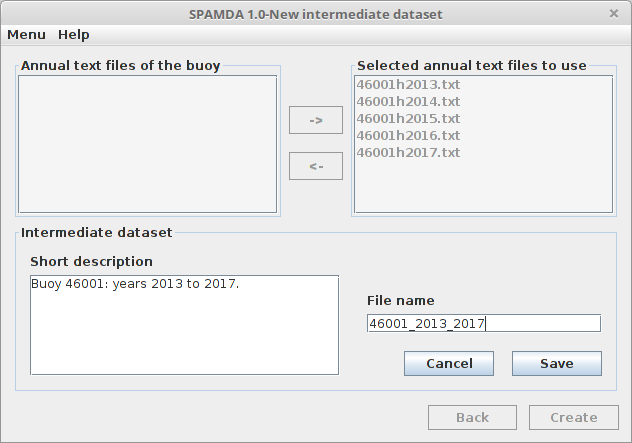
\includegraphics[scale=0.43]{figures/creatingIntermediateDataset_CS.png}
				\caption{New intermediate dataset view.}\label{fig:intermediate}
			\end{figure}
			
			Here the researcher can select the annual text files that he wants to include in the intermediate dataset by clicking on the \textcolor{blue}{\textit{$-$$>$}} button (click on the \textcolor{blue}{\textit{$<$$-$}} button to deselect a previously selected one). In this case, all the files introduced before which correspond to the buoy under study were selected. When the files selection is finished, \textcolor{blue}{\textit{Create}} button will be clicked in order to be able to introduce the description and the file name of the current intermediate dataset, and then clicking on the \textcolor{blue}{\textit{Save}} button, the creation process will start, and the application will show the status of such process.
			
			\begin{figure}[ht!]
				\centering
				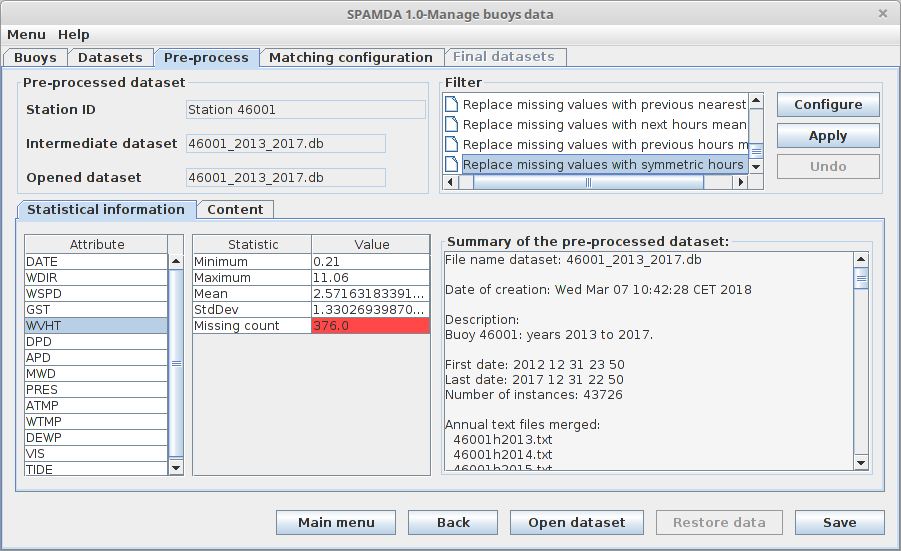
\includegraphics[scale=0.40]{figures/tabPreprocess_CS.png}
				\caption{Tab \textit{Pre-process}.}\label{fig:preprocess_data}
			\end{figure}
			
			%After that, in order to prepare the intermediate dataset to be able to be used by ML algorithms correctly, the dataset to be prepared is selected, and then the button \textcolor{blue}{\textit{Open}} is clicked to jump to the tab \textcolor{blue}{\textit{Pre-process}} (represented in Figure \ref{fig:preprocess_data}). In this tab, relevant statistical information about the selected dataset is shown, and also the content of the dataset can be consulted, providing the researcher the capacity to evaluate the pre-processing being performed.
			
			After that, in order to prepare the intermediate dataset to be able to be used by ML algorithms correctly, the dataset to be prepared is selected, and then the button \textcolor{blue}{\textit{Open}} is clicked to jump to the tab \textcolor{blue}{\textit{Pre-process}} (represented in Figure \ref{fig:preprocess_data}).

			%As mentioned at the beginning of this chapter, this case study will process the data to be ready to classify waves considering their height, so any missing data from wave height ($376$ values) was recovered and some filters were applied to the remaining variables. After finishing the pre-processing of the dataset, the researcher can click on the \textcolor{blue}{\textit{Save}} button, to introduce the description and file name for the current pre-processed dataset.
			
			As mentioned at the beginning of this chapter, this case study will process the data to be ready to classify waves considering their height, so any missing data from wave height ($376$ values) and the remaining attributes are recovered, using the filter \textit{Replace missing values with symmetric $3$ hours mean}. Furthermore, the attributes MWD, DEWP, VIS and TIDE are removed from the dataset by applying the filter \textit{RemoveByName}, since the first two had more than $92$\% of missing data and the last two $100$\%. After finishing the pre-processing of the dataset, the researcher can click on the \textcolor{blue}{\textit{Save}} button, to introduce the description and file name for the current pre-processed dataset.
			
			At this point, the researcher has registered the buoy in SPAMDA, then entered its raw data and selected the required data for the problem (intermediate dataset), finally, the data was pre-processed in order to be ready for its future use in ML algorithms. In order to achieve a more accurate description of the problem under study, a matching process can be carried out to merge the processed data from NDBC with the reanalysis data (also entered previously) from NNRP. The next step is to click on the \textcolor{blue}{\textit{Matching configuration}} tab, to open the view shown in  Figure \ref{fig:matching_conf}. 
			
			\begin{figure}[ht!]
				\centering
				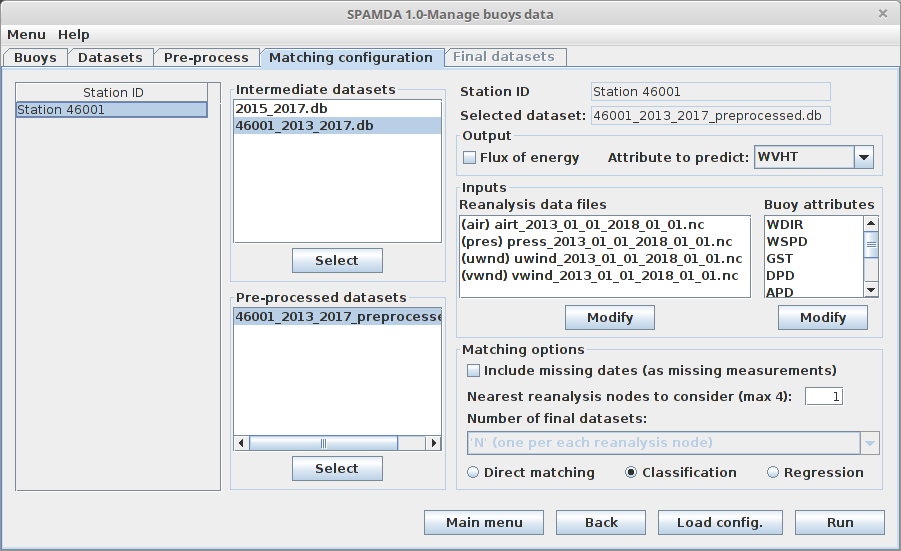
\includegraphics[scale=0.40]{figures/tabMatchingConfiguration_CS.png}
				\caption{Tab \textit{Matching configuration}.}\label{fig:matching_conf}
			\end{figure}
			
			In this view, the researcher can customise (or load) the parameters of the matching process according to his needs, and select the prediction task (described in Section \ref{sec:MatchingConf}) that the final dataset will be used in. For this example the pre-processed dataset created and the following parameters were selected:
			\begin{itemize}
				\setlength\itemsep{0.01cm}
				\item \textit{\textbf{Attribute to predict}}: WVHT.
				\item \textit{\textbf{Reanalysis data}}: Air, pressure, u-wind and v-wind.
				\item \textit{\textbf{Buoy attributes to be used as inputs}}: WDIR, WSPD, GST, DPD, APD, PRES, ATMP and WTMP.
				\item \textit{\textbf{Reanalysis nodes to consider}}: $1$.
				\item \textit{\textbf{Number of final datasets}}: In this example that option is disabled because only 1 reanalysis node is considered.
				\item \textit{\textbf{Prediction task}}: Classification.
			\end{itemize} 

			After configuring the matching process, the researcher can click on the \textcolor{blue}{\textit{Run}} button to jump to the view shown in Figure \ref{fig:final_dataset} and proceed to define the final dataset structure according to the selected prediction task.
			
			\begin{figure}[ht!]
				\centering
				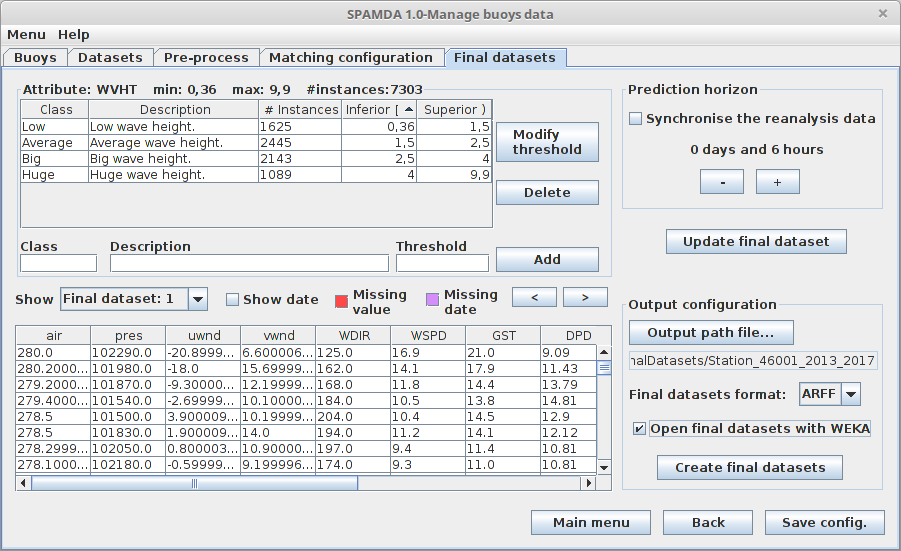
\includegraphics[scale=0.40]{figures/tabFinalDatasets_CS.png}
				\caption{Tab \textit{Final datasets}.}\label{fig:final_dataset}
			\end{figure}
			
			As in the previous window \textit{Classification} was selected, now the researcher is able to add, modify or delete the thresholds (usually defined by an expert) used to discretise the output variable. After adding the necessary thresholds, the next step is to set the time horizon desired and also to activate (if desired) the synchronisation (in time) of reanalysis variables with the output one as explained in Section {\ref{sec:FinalDatasets}}. Then the researcher would click on the \textcolor{blue}{\textit{Update final dataset}} button to see the content of the final dataset which is shown in the bottom left corner and finally, after checking that everything is correct, the last step would be to select the name (and path) of the dataset file, its output format and click on the \textcolor{blue}{\textit{Create final datasets}} button. For this case study the following configuration was applied:
			\vspace{-0.25cm}
			\begin{table}[ht!]
			
				\caption{Defined thresholds.}
				\label{tab:thresholds}
				\footnotesize
				\centering

				\begin{tabular}{cm{3.20cm}cc@{\setlength{\tabcolsep}{0pt}}m{0.0cm}}
				
					\cline{1-5}
					
					\textbf{Class}&\textbf{Description}&\textbf{Inferior [}&\textbf{Superior )}&\\[0.20cm]

					\cline{1-5}
					
					Low & Low wave height & $0.36$ & $1.5$&\\[0.15cm]
					
					\cellcolor{gray090}Average & \cellcolor{gray090}Average wave height & \cellcolor{gray090}$1.5$ & \cellcolor{gray090}$2.5$&\\[0.15cm]
					
					Big & Big wave height & $2.5$ & $4.0$&\\[0.15cm]
					
					\cellcolor{gray090}Huge & \cellcolor{gray090}Huge wave height & \cellcolor{gray090}$4.0$ & \cellcolor{gray090}$9.9$&\\[0.02cm]

					\cline{1-5}
						
				\end{tabular}
			
			\end{table}

			\begin{itemize}
				\item Thresholds: see in Table \ref{tab:thresholds}.
				\item Prediction horizon: 6 hours
				\item Synchronisation: Disabled
			\end{itemize}
			
			At this point the final dataset would be created and stored in the computer of the researcher. Also there is an option to open the dataset with WEKA (after creating it) in order to perform a first classification approach or a preliminary study of the data structure, as shown in Fig. \ref{fig:openigFinalDatasetWekaCE}.

			\begin{figure}[ht!]
				\centering
				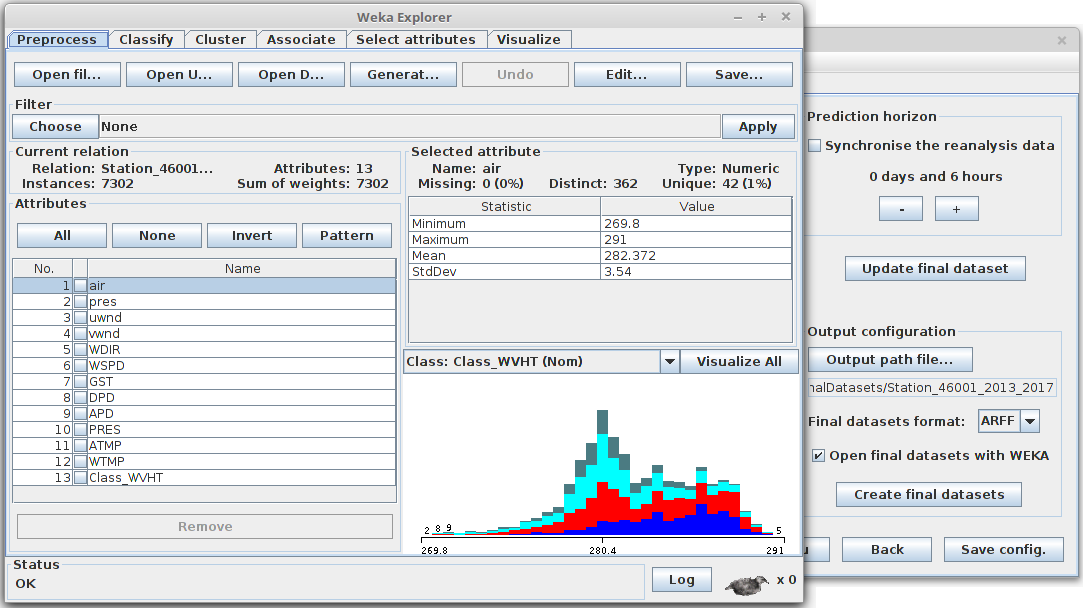
\includegraphics[scale=0.39]{figures/openigFinalDatasetWekaCE.png}
				\caption{The final dataset opened with the environment Explorer of WEKA.}
				\label{fig:openigFinalDatasetWekaCE}
			\end{figure}

	\end{onehalfspace}
	

	% Licencia de SPAMDA.
	
\chapter{License of SPAMDA}

	\begin{onehalfspace}
	
		A copy of the license of SPAMDA regarding the use and distribution of the source code and binary is included in the appendix entitled "License of SPAMDA" \ref{licenseGPLSPAMDA}.

	\end{onehalfspace}

	
	% Agradecimientos.
	
\chapter{Acknowledgments}

	\begin{onehalfspace}
	
		This work has been partially subsidised by the projects TIN2017-85887-C2-1-P and TIN2017-90567-REDT of the Spanish Ministry of Economy and Competitiveness (MI\-NE\-CO), and FEDER funds of the European Union. We also thank to NVIDIA Corporation for the transfer of computational resources for research works.
	
		The authors thank to NOAA/OAR/ESRL PSD, Boulder, Colorado, USA for the NCEP Reanalysis data provided from their Web site at https://www.esrl.noaa.gov/psd/, and to NOAA/NDBC by its data that were collected and made freely available.
		
		We also thank to University of Waikato for the Weka (Waikato Environment for Knowledge Analysis) software tool, to University Corporation for Atmospheric Research/Unidata for the NetCDF (network Common Data Form) Java library and to QOS.ch for the SLF4J (Simple Logging Facade for Java) library.
	
	\end{onehalfspace}


	% La bibliografía aparecerá al mismo nivel que el resto de capítulos.
	\bookmarksetup{startatroot}

		% Página en blanco
		\paginavaciacompleta
		
		% Se inserta la bibliografía.
		\bibliography{bib/bibfile}
		
		
	% Apéndice con los pasos para obtener los ficheros del NDBC y NNRP y cada una de las licencias.
	\appendix
		\appendixpage
		\addappheadtotoc
		
		% Paso para obtener los ficheros del NDBC y NNRP.
		
\chapter{Getting meteorological data}\label{app:GettingMetData}

	\begin{onehalfspace}
	
		%	Formato con ejemplo y capturas:
		
		\section{Getting an annual text file from NDBC}

			The following steps shows the procedure to obtain an annual text file that contain the measurements collected by a buoy from NDBC, concretely the file of the year $2017$ corresponding to the buoy identified as \textit{Station 46001}, moored at Western Gulf of Alaska.
			
				\begin{itemize}
					%\setlength\itemsep{0.01cm}
					\item \textit{\textbf{Step 1}}: Open the web browser and visit the NDBC web page \cite{NOAA_1}.
					\item \textit{\textbf{Step 2}}: Navigate to the desired buoy and click on the year to download (see Fig. \ref{fig:selectingBuoy}).
						\begin{figure}[ht!]
							\centering
							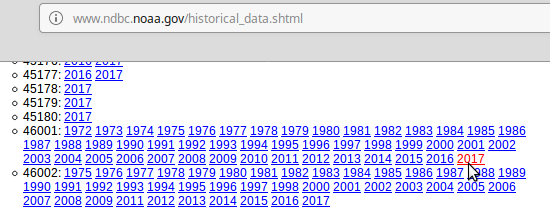
\includegraphics[scale=0.48]{figures/selectingBuoy.png}
							\caption{Selecting the desired buoy and year.}
							\label{fig:selectingBuoy}
						\end{figure}
					\item \textit{\textbf{Step 3}}: In the option \textit{\textbf{Method Two}} click on the file (see Fig. \ref{fig:downloadingTextFile}) and its content will be shown.
						\begin{figure}[ht!]
							\centering
							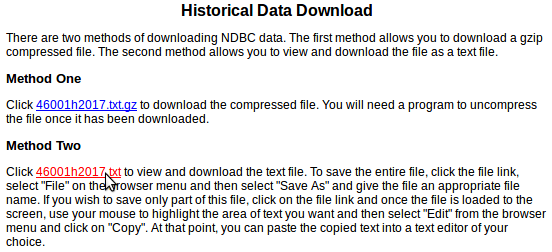
\includegraphics[scale=0.48]{figures/downloadingTextFile.png}
							\caption{Downloading the annual text file.}
							\label{fig:downloadingTextFile}
						\end{figure}
					\item \textit{\textbf{Step 4}}: In the menu bar of the web browser select \textit{\textbf{File}} and \textit{\textbf{Save As}} to save the file in the computer.
				\end{itemize}
			
		\section{Getting a reanalysis data file from NNRP}
		
			%	Formato con ejemplo y capturas:

			The following steps shows the procedure to obtain a reanalysis data file from NNRP, concretely for the variable \textit{Air temperature} and corresponding to the year $2017$ and the reanalysis nodes $57.5$ N $\times$ $147.5$ W, $57.5$ N $\times$ $150.0$ W, $57.5$ N $\times$ $152.5$ W, $55.0$ N $\times$ $147.5$ W, $55.0$ N $\times$ $150.0$ W and $55.0$ N $\times$ $152.5$ W.
			
				\begin{itemize}
					%\setlength\itemsep{0.01cm}
					\item \textit{\textbf{Step 1}}: Open the web browser and visit the NNRP  web page \cite{NNRP}.
					\item \textit{\textbf{Step 2}}: Navigate to the \textit{\textbf{Surface}} section and click on it (see Fig. \ref{fig:selectingSurfaceSection}).
						\begin{figure}[ht!]
							\centering
							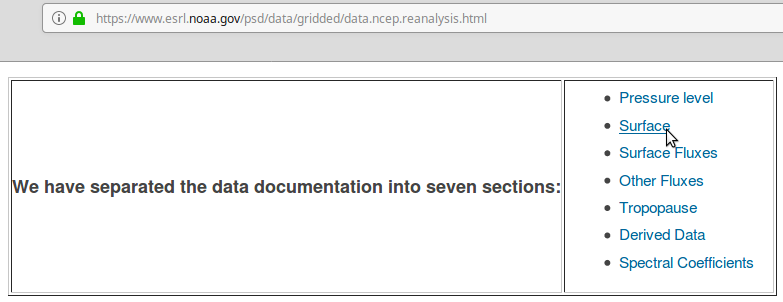
\includegraphics[scale=0.40]{figures/selectingSurfaceSection.png}
							\caption{Selecting \textit{\textbf{Surface}} section.}
							\label{fig:selectingSurfaceSection}
						\end{figure}
					\item \textit{\textbf{Step 3}}: Navigate to the \textit{\textbf{Update Schedule}} section, search for the statistic \textit{\textbf{4-times Daily}} of the desired variable and click on the image for creating a plot or subset (see Fig. \ref{fig:selectingVariable}).
						\begin{figure}[ht!]
							\centering
							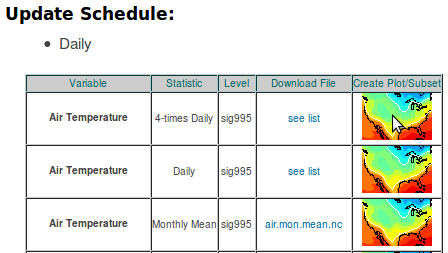
\includegraphics[scale=0.55]{figures/selectingVariable.png}
							\caption{Selecting reanalysis variable.}
							\label{fig:selectingVariable}
						\end{figure}
					\item \textit{\textbf{Step 4}}: Navigate to the \textit{\textbf{Surface}} level and click on \textit{\textbf{Make plot or subset}} (see Fig. \ref{fig:selectingMakePlot}).
						\begin{figure}[ht!]
							\centering
							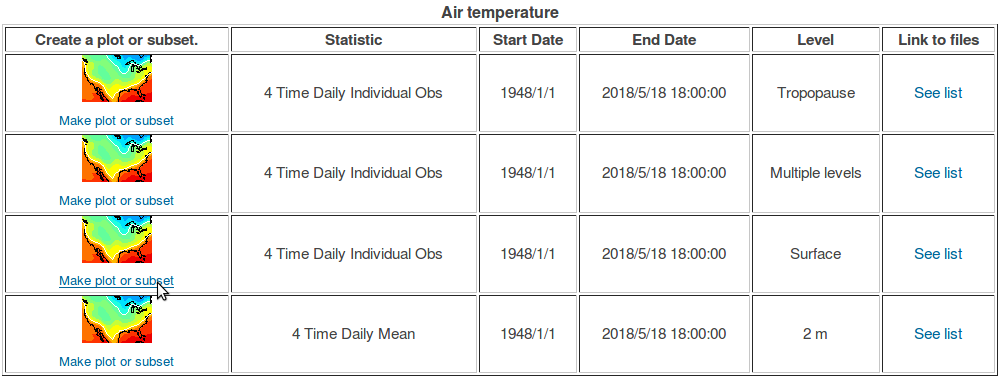
\includegraphics[scale=0.42]{figures/selectingMakePlot.png}
							\caption{Selecting \textit{\textbf{Make plot or subset}.}}
							\label{fig:selectingMakePlot}
						\end{figure}
					\item \textit{\textbf{Step 5}}: In the new web page that has been appeared do the following (see Fig. \ref{fig:selectingProperties.png}):
						\begin{itemize}
							\item In \textit{\textbf{Axis Dimensions}} type the desired sub-grid (spatial properties).
							\item In \textit{\textbf{Other dimension value(s)}} type the desired ranges of dates (temporal properties).
							\item In \textit{\textbf{Output options}} select the option \textit{Create a subset without making a plot}.
							\item Click on \textit{\textbf{Create Plot or Subset of Data}} button (at bottom of the web page) to generate the reanalysis data file with the desired properties.
						\end{itemize}
% 						\begin{figure}[ht!]
% 							\centering
% 							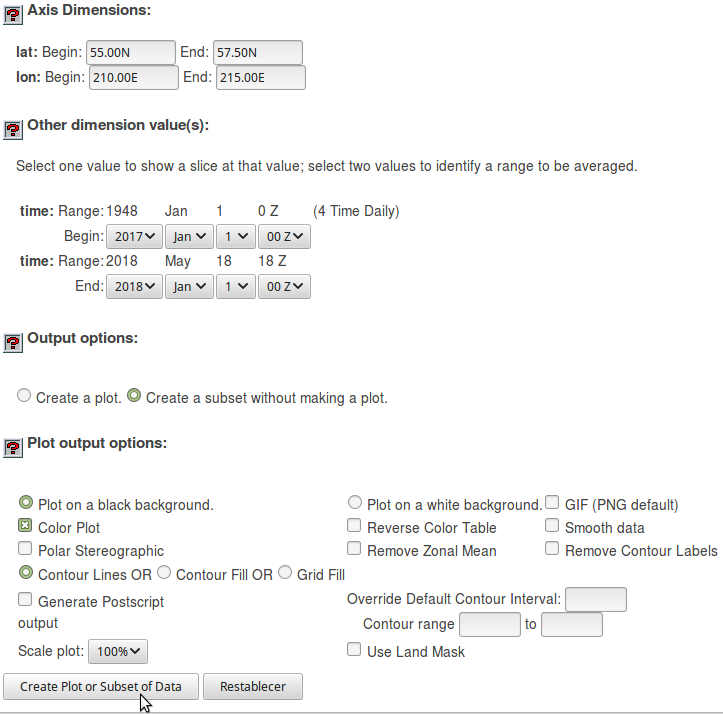
\includegraphics[scale=0.50]{figures/selectingProperties.png}
% 							\caption{Typing desired properties of the file to get.}
% 							\label{fig:selectingProperties.png}
% 						\end{figure}
					\item \textit{\textbf{Step 6}}: Finally click on \textit{\textbf{FTP a copy of the file}} button to download the reanalysis data file on the computer.
				\end{itemize}
				
				\begin{figure}[ht!]
					\centering
					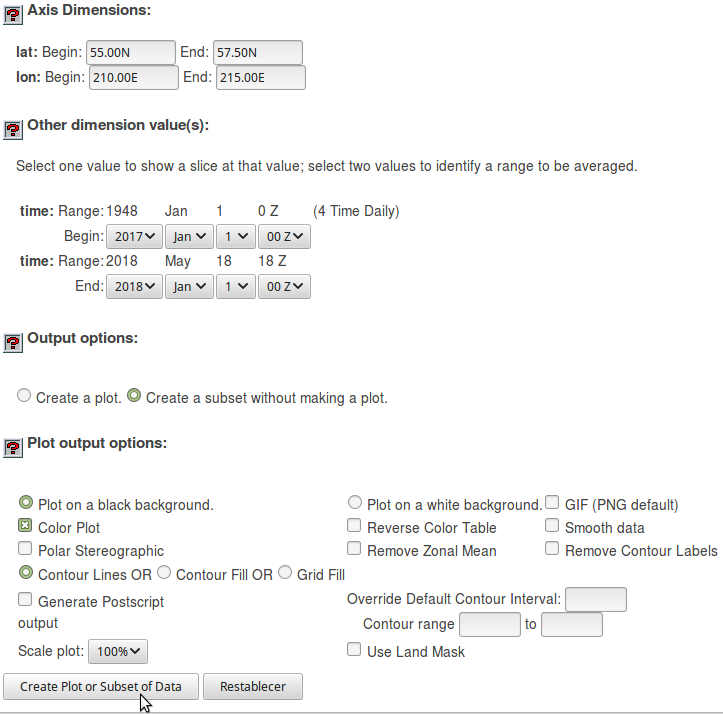
\includegraphics[scale=0.50]{figures/selectingProperties.png}
					\caption{Typing desired properties of the file to get.}
					\label{fig:selectingProperties.png}
				\end{figure}
				
				\clearpage
				
	\end{onehalfspace}
	
%	Formato abreviado:

%	Follow these steps to obtain an annual text file that contain the measurements collected by a buoy from NDBC:
%		\begin{itemize}
%			\item \textit{\textbf{Step 1}}: Open the web browser and visit the NDBC web page \cite{NOAA_1}.
%			\item \textit{\textbf{Step 2}}: Navigate to the desired buoy and click on the year to download.
%			\item \textit{\textbf{Step 3}}: In the option \textit{\textbf{Method Two}} click on the file and its content will be shown.
%			\item \textit{\textbf{Step 4}}: In the menu bar of the web browser select \textit{\textbf{File}} and \textit{\textbf{Save As}} to save it in the computer.
%		\end{itemize}	

%	Formato abreviado:
		
%	Follow these steps to obtain a reanalysis data file from NNRP:
%	
%		\begin{itemize}
%			\item \textit{\textbf{Step 1}}: Open the web browser and visit the NNRP  web page \cite{NNRP}.
%			\item \textit{\textbf{Step 2}}: Navigate to the \textit{\textbf{Surface}} section and click on it.
%			\item \textit{\textbf{Step 3}}: Navigate to the \textit{\textbf{Update Schedule}} section, search for the statistic \textit{\textbf{4-times Daily}} of the desired variable and click on the image for creating a plot or subset.
%			\item \textit{\textbf{Step 4}}: Navigate to the \textit{\textbf{Surface}} level and click on \textit{\textbf{Make plot or subset}}.
%			\item \textit{\textbf{Step 5}}: In the new web page that has been appeared do the following:
%				\begin{itemize}
%					\item In \textit{\textbf{Axis Dimensions}} type the desired grid (spatial properties).
%					\item In \textit{\textbf{Other dimension value(s)}} type the desired ranges of dates (temporal properties).
%					\item In \textit{\textbf{Output options}} select the option \textit{Create a subset without making a plot}.
%					\item Click on \textit{\textbf{Create Plot or Subset of Data}} button (bottom of the web page) to generate the reanalysis data file with the desired properties.
%				\end{itemize}
%			\item \textit{\textbf{Step 6}}: Finally click on \textit{\textbf{FTP a copy of the file}} button to download the reanalysis data file on the computer.
%		\end{itemize}

		
		% Página en blanco
		\paginavaciacompleta
		
		% Licencia de la documentación de FSF.
		% This is set up to run with pdflatex.
%---------The file header---------------------------------------------
%\documentclass[a4paper,12pt]{book}

%\usepackage[english]{babel} %language selection
%\selectlanguage{english}

%\pagenumbering{arabic}

%\usepackage{hyperref}
%\hypersetup{colorlinks, 
%           citecolor=black,
%           filecolor=black,
%           linkcolor=black,
%           urlcolor=black,
%           bookmarksopen=true,
%           pdftex}

%\hfuzz = .6pt % avoid black boxes
           
%\begin{document}
%---------------------------------------------------------------------
\fancyhead[LO]{GNU Free Documentation License}
\fancyhead[RE]{GNU Free Documentation License}
%\chapter*{\rlap{GNU Free Documentation License}} \label{GFDL_LICENSE}
%\phantomsection  % so hyperref creates bookmarks
%\addcontentsline{toc}{chapter}{GNU Free Documentation License}
\chapter{GNU Free Documentation License} \label{GFDL_LICENSE}
%\fancyhead[L]{GNU Free Documentation License}
%\label{label_fdl}

 \begin{center}

       Version 1.3, 3 November 2008


 Copyright \copyright{} 2000, 2001, 2002, 2007, 2008  Free Software Foundation, Inc.
 
 \bigskip
 
     \texttt{<https://fsf.org/>}
  
 \bigskip
 
 Everyone is permitted to copy and distribute verbatim copies
 of this license document, but changing it is not allowed.
\end{center}


\begin{center}
{\bf\large Preamble}
\end{center}

The purpose of this License is to make a manual, textbook, or other
functional and useful document ``free'' in the sense of freedom: to
assure everyone the effective freedom to copy and redistribute it,
with or without modifying it, either commercially or noncommercially.
Secondarily, this License preserves for the author and publisher a way
to get credit for their work, while not being considered responsible
for modifications made by others.

This License is a kind of ``copyleft'', which means that derivative
works of the document must themselves be free in the same sense.  It
complements the GNU General Public License, which is a copyleft
license designed for free software.

We have designed this License in order to use it for manuals for free
software, because free software needs free documentation: a free
program should come with manuals providing the same freedoms that the
software does.  But this License is not limited to software manuals;
it can be used for any textual work, regardless of subject matter or
whether it is published as a printed book.  We recommend this License
principally for works whose purpose is instruction or reference.


\begin{center}
{\Large\bf 1. APPLICABILITY AND DEFINITIONS\par}
\phantomsection
\addcontentsline{toc}{section}{1. APPLICABILITY AND DEFINITIONS}
\end{center}

This License applies to any manual or other work, in any medium, that
contains a notice placed by the copyright holder saying it can be
distributed under the terms of this License.  Such a notice grants a
world-wide, royalty-free license, unlimited in duration, to use that
work under the conditions stated herein.  The ``\textbf{Document}'', below,
refers to any such manual or work.  Any member of the public is a
licensee, and is addressed as ``\textbf{you}''.  You accept the license if you
copy, modify or distribute the work in a way requiring permission
under copyright law.

A ``\textbf{Modified Version}'' of the Document means any work containing the
Document or a portion of it, either copied verbatim, or with
modifications and/or translated into another language.

A ``\textbf{Secondary Section}'' is a named appendix or a front-matter section of
the Document that deals exclusively with the relationship of the
publishers or authors of the Document to the Document's overall subject
(or to related matters) and contains nothing that could fall directly
within that overall subject.  (Thus, if the Document is in part a
textbook of mathematics, a Secondary Section may not explain any
mathematics.)  The relationship could be a matter of historical
connection with the subject or with related matters, or of legal,
commercial, philosophical, ethical or political position regarding
them.

The ``\textbf{Invariant Sections}'' are certain Secondary Sections whose titles
are designated, as being those of Invariant Sections, in the notice
that says that the Document is released under this License.  If a
section does not fit the above definition of Secondary then it is not
allowed to be designated as Invariant.  The Document may contain zero
Invariant Sections.  If the Document does not identify any Invariant
Sections then there are none.

The ``\textbf{Cover Texts}'' are certain short passages of text that are listed,
as Front-Cover Texts or Back-Cover Texts, in the notice that says that
the Document is released under this License.  A Front-Cover Text may
be at most 5 words, and a Back-Cover Text may be at most 25 words.

A ``\textbf{Transparent}'' copy of the Document means a machine-readable copy,
represented in a format whose specification is available to the
general public, that is suitable for revising the document
straightforwardly with generic text editors or (for images composed of
pixels) generic paint programs or (for drawings) some widely available
drawing editor, and that is suitable for input to text formatters or
for automatic translation to a variety of formats suitable for input
to text formatters.  A copy made in an otherwise Transparent file
format whose markup, or absence of markup, has been arranged to thwart
or discourage subsequent modification by readers is not Transparent.
An image format is not Transparent if used for any substantial amount
of text.  A copy that is not ``Transparent'' is called ``\textbf{Opaque}''.

Examples of suitable formats for Transparent copies include plain
ASCII without markup, Texinfo input format, LaTeX input format, SGML
or XML using a publicly available DTD, and standard-conforming simple
HTML, PostScript or PDF designed for human modification.  Examples of
transparent image formats include PNG, XCF and JPG.  Opaque formats
include proprietary formats that can be read and edited only by
proprietary word processors, SGML or XML for which the DTD and/or
processing tools are not generally available, and the
machine-generated HTML, PostScript or PDF produced by some word
processors for output purposes only.

The ``\textbf{Title Page}'' means, for a printed book, the title page itself,
plus such following pages as are needed to hold, legibly, the material
this License requires to appear in the title page.  For works in
formats which do not have any title page as such, ``Title Page'' means
the text near the most prominent appearance of the work's title,
preceding the beginning of the body of the text.

The ``\textbf{publisher}'' means any person or entity that distributes
copies of the Document to the public.

A section ``\textbf{Entitled XYZ}'' means a named subunit of the Document whose
title either is precisely XYZ or contains XYZ in parentheses following
text that translates XYZ in another language.  (Here XYZ stands for a
specific section name mentioned below, such as ``\textbf{Acknowledgements}'',
``\textbf{Dedications}'', ``\textbf{Endorsements}'', or ``\textbf{History}''.)  
To ``\textbf{Preserve the Title}''
of such a section when you modify the Document means that it remains a
section ``Entitled XYZ'' according to this definition.

The Document may include Warranty Disclaimers next to the notice which
states that this License applies to the Document.  These Warranty
Disclaimers are considered to be included by reference in this
License, but only as regards disclaiming warranties: any other
implication that these Warranty Disclaimers may have is void and has
no effect on the meaning of this License.


\begin{center}
{\Large\bf 2. VERBATIM COPYING\par}
\phantomsection
\addcontentsline{toc}{section}{2. VERBATIM COPYING}
\end{center}

You may copy and distribute the Document in any medium, either
commercially or noncommercially, provided that this License, the
copyright notices, and the license notice saying this License applies
to the Document are reproduced in all copies, and that you add no other
conditions whatsoever to those of this License.  You may not use
technical measures to obstruct or control the reading or further
copying of the copies you make or distribute.  However, you may accept
compensation in exchange for copies.  If you distribute a large enough
number of copies you must also follow the conditions in section~3.

You may also lend copies, under the same conditions stated above, and
you may publicly display copies.


\begin{center}
{\Large\bf 3. COPYING IN QUANTITY\par}
\phantomsection
\addcontentsline{toc}{section}{3. COPYING IN QUANTITY}
\end{center}


If you publish printed copies (or copies in media that commonly have
printed covers) of the Document, numbering more than 100, and the
Document's license notice requires Cover Texts, you must enclose the
copies in covers that carry, clearly and legibly, all these Cover
Texts: Front-Cover Texts on the front cover, and Back-Cover Texts on
the back cover.  Both covers must also clearly and legibly identify
you as the publisher of these copies.  The front cover must present
the full title with all words of the title equally prominent and
visible.  You may add other material on the covers in addition.
Copying with changes limited to the covers, as long as they preserve
the title of the Document and satisfy these conditions, can be treated
as verbatim copying in other respects.

If the required texts for either cover are too voluminous to fit
legibly, you should put the first ones listed (as many as fit
reasonably) on the actual cover, and continue the rest onto adjacent
pages.

If you publish or distribute Opaque copies of the Document numbering
more than 100, you must either include a machine-readable Transparent
copy along with each Opaque copy, or state in or with each Opaque copy
a computer-network location from which the general network-using
public has access to download using public-standard network protocols
a complete Transparent copy of the Document, free of added material.
If you use the latter option, you must take reasonably prudent steps,
when you begin distribution of Opaque copies in quantity, to ensure
that this Transparent copy will remain thus accessible at the stated
location until at least one year after the last time you distribute an
Opaque copy (directly or through your agents or retailers) of that
edition to the public.

It is requested, but not required, that you contact the authors of the
Document well before redistributing any large number of copies, to give
them a chance to provide you with an updated version of the Document.


\begin{center}
{\Large\bf 4. MODIFICATIONS\par}
\phantomsection
\addcontentsline{toc}{section}{4. MODIFICATIONS}
\end{center}

You may copy and distribute a Modified Version of the Document under
the conditions of sections 2 and 3 above, provided that you release
the Modified Version under precisely this License, with the Modified
Version filling the role of the Document, thus licensing distribution
and modification of the Modified Version to whoever possesses a copy
of it.  In addition, you must do these things in the Modified Version:

\begin{itemize}
\item[A.] 
   Use in the Title Page (and on the covers, if any) a title distinct
   from that of the Document, and from those of previous versions
   (which should, if there were any, be listed in the History section
   of the Document).  You may use the same title as a previous version
   if the original publisher of that version gives permission.
   
\item[B.]
   List on the Title Page, as authors, one or more persons or entities
   responsible for authorship of the modifications in the Modified
   Version, together with at least five of the principal authors of the
   Document (all of its principal authors, if it has fewer than five),
   unless they release you from this requirement.
   
\item[C.]
   State on the Title page the name of the publisher of the
   Modified Version, as the publisher.
   
\item[D.]
   Preserve all the copyright notices of the Document.
   
\item[E.]
   Add an appropriate copyright notice for your modifications
   adjacent to the other copyright notices.
   
\item[F.]
   Include, immediately after the copyright notices, a license notice
   giving the public permission to use the Modified Version under the
   terms of this License, in the form shown in the Addendum below.
   
\item[G.]
   Preserve in that license notice the full lists of Invariant Sections
   and required Cover Texts given in the Document's license notice.
   
\item[H.]
   Include an unaltered copy of this License.
   
\item[I.]
   Preserve the section Entitled ``History'', Preserve its Title, and add
   to it an item stating at least the title, year, new authors, and
   publisher of the Modified Version as given on the Title Page.  If
   there is no section Entitled ``History'' in the Document, create one
   stating the title, year, authors, and publisher of the Document as
   given on its Title Page, then add an item describing the Modified
   Version as stated in the previous sentence.
   
\item[J.]
   Preserve the network location, if any, given in the Document for
   public access to a Transparent copy of the Document, and likewise
   the network locations given in the Document for previous versions
   it was based on.  These may be placed in the ``History'' section.
   You may omit a network location for a work that was published at
   least four years before the Document itself, or if the original
   publisher of the version it refers to gives permission.
   
\item[K.]
   For any section Entitled ``Acknowledgements'' or ``Dedications'',
   Preserve the Title of the section, and preserve in the section all
   the substance and tone of each of the contributor acknowledgements
   and/or dedications given therein.
   
\item[L.]
   Preserve all the Invariant Sections of the Document,
   unaltered in their text and in their titles.  Section numbers
   or the equivalent are not considered part of the section titles.
   
\item[M.]
   Delete any section Entitled ``Endorsements''.  Such a section
   may not be included in the Modified Version.
   
\item[N.]
   Do not retitle any existing section to be Entitled ``Endorsements''
   or to conflict in title with any Invariant Section.
   
\item[O.]
   Preserve any Warranty Disclaimers.
\end{itemize}

If the Modified Version includes new front-matter sections or
appendices that qualify as Secondary Sections and contain no material
copied from the Document, you may at your option designate some or all
of these sections as invariant.  To do this, add their titles to the
list of Invariant Sections in the Modified Version's license notice.
These titles must be distinct from any other section titles.

You may add a section Entitled ``Endorsements'', provided it contains
nothing but endorsements of your Modified Version by various
parties---for example, statements of peer review or that the text has
been approved by an organization as the authoritative definition of a
standard.

You may add a passage of up to five words as a Front-Cover Text, and a
passage of up to 25 words as a Back-Cover Text, to the end of the list
of Cover Texts in the Modified Version.  Only one passage of
Front-Cover Text and one of Back-Cover Text may be added by (or
through arrangements made by) any one entity.  If the Document already
includes a cover text for the same cover, previously added by you or
by arrangement made by the same entity you are acting on behalf of,
you may not add another; but you may replace the old one, on explicit
permission from the previous publisher that added the old one.

The author(s) and publisher(s) of the Document do not by this License
give permission to use their names for publicity for or to assert or
imply endorsement of any Modified Version.


\begin{center}
{\Large\bf 5. COMBINING DOCUMENTS\par}
\phantomsection
\addcontentsline{toc}{section}{5. COMBINING DOCUMENTS}
\end{center}


You may combine the Document with other documents released under this
License, under the terms defined in section~4 above for modified
versions, provided that you include in the combination all of the
Invariant Sections of all of the original documents, unmodified, and
list them all as Invariant Sections of your combined work in its
license notice, and that you preserve all their Warranty Disclaimers.

The combined work need only contain one copy of this License, and
multiple identical Invariant Sections may be replaced with a single
copy.  If there are multiple Invariant Sections with the same name but
different contents, make the title of each such section unique by
adding at the end of it, in parentheses, the name of the original
author or publisher of that section if known, or else a unique number.
Make the same adjustment to the section titles in the list of
Invariant Sections in the license notice of the combined work.

In the combination, you must combine any sections Entitled ``History''
in the various original documents, forming one section Entitled
``History''; likewise combine any sections Entitled ``Acknowledgements'',
and any sections Entitled ``Dedications''.  You must delete all sections
Entitled ``Endorsements''.

\begin{center}
{\Large\bf 6. COLLECTIONS OF DOCUMENTS\par}
\phantomsection
\addcontentsline{toc}{section}{6. COLLECTIONS OF DOCUMENTS}
\end{center}

You may make a collection consisting of the Document and other documents
released under this License, and replace the individual copies of this
License in the various documents with a single copy that is included in
the collection, provided that you follow the rules of this License for
verbatim copying of each of the documents in all other respects.

You may extract a single document from such a collection, and distribute
it individually under this License, provided you insert a copy of this
License into the extracted document, and follow this License in all
other respects regarding verbatim copying of that document.


\begin{center}
{\Large\bf 7. AGGREGATION WITH INDEPENDENT WORKS\par}
\phantomsection
\addcontentsline{toc}{section}{7. AGGREGATION WITH INDEPENDENT WORKS}
\end{center}


A compilation of the Document or its derivatives with other separate
and independent documents or works, in or on a volume of a storage or
distribution medium, is called an ``aggregate'' if the copyright
resulting from the compilation is not used to limit the legal rights
of the compilation's users beyond what the individual works permit.
When the Document is included in an aggregate, this License does not
apply to the other works in the aggregate which are not themselves
derivative works of the Document.

If the Cover Text requirement of section~3 is applicable to these
copies of the Document, then if the Document is less than one half of
the entire aggregate, the Document's Cover Texts may be placed on
covers that bracket the Document within the aggregate, or the
electronic equivalent of covers if the Document is in electronic form.
Otherwise they must appear on printed covers that bracket the whole
aggregate.


\begin{center}
{\Large\bf 8. TRANSLATION\par}
\phantomsection
\addcontentsline{toc}{section}{8. TRANSLATION}
\end{center}


Translation is considered a kind of modification, so you may
distribute translations of the Document under the terms of section~4.
Replacing Invariant Sections with translations requires special
permission from their copyright holders, but you may include
translations of some or all Invariant Sections in addition to the
original versions of these Invariant Sections.  You may include a
translation of this License, and all the license notices in the
Document, and any Warranty Disclaimers, provided that you also include
the original English version of this License and the original versions
of those notices and disclaimers.  In case of a disagreement between
the translation and the original version of this License or a notice
or disclaimer, the original version will prevail.

If a section in the Document is Entitled ``Acknowledgements'',
``Dedications'', or ``History'', the requirement (section~4) to Preserve
its Title (section~1) will typically require changing the actual
title.


\begin{center}
{\Large\bf 9. TERMINATION\par}
\phantomsection
\addcontentsline{toc}{section}{9. TERMINATION}
\end{center}


You may not copy, modify, sublicense, or distribute the Document
except as expressly provided under this License.  Any attempt
otherwise to copy, modify, sublicense, or distribute it is void, and
will automatically terminate your rights under this License.

However, if you cease all violation of this License, then your license
from a particular copyright holder is reinstated (a) provisionally,
unless and until the copyright holder explicitly and finally
terminates your license, and (b) permanently, if the copyright holder
fails to notify you of the violation by some reasonable means prior to
60 days after the cessation.

Moreover, your license from a particular copyright holder is
reinstated permanently if the copyright holder notifies you of the
violation by some reasonable means, this is the first time you have
received notice of violation of this License (for any work) from that
copyright holder, and you cure the violation prior to 30 days after
your receipt of the notice.

Termination of your rights under this section does not terminate the
licenses of parties who have received copies or rights from you under
this License.  If your rights have been terminated and not permanently
reinstated, receipt of a copy of some or all of the same material does
not give you any rights to use it.


\begin{center}
{\Large\bf 10. FUTURE REVISIONS OF THIS LICENSE\par}
\phantomsection
\addcontentsline{toc}{section}{10. FUTURE REVISIONS OF THIS LICENSE}
\end{center}


The Free Software Foundation may publish new, revised versions
of the GNU Free Documentation License from time to time.  Such new
versions will be similar in spirit to the present version, but may
differ in detail to address new problems or concerns.  See
\texttt{https://www.gnu.org/licenses/}.

Each version of the License is given a distinguishing version number.
If the Document specifies that a particular numbered version of this
License ``or any later version'' applies to it, you have the option of
following the terms and conditions either of that specified version or
of any later version that has been published (not as a draft) by the
Free Software Foundation.  If the Document does not specify a version
number of this License, you may choose any version ever published (not
as a draft) by the Free Software Foundation.  If the Document
specifies that a proxy can decide which future versions of this
License can be used, that proxy's public statement of acceptance of a
version permanently authorizes you to choose that version for the
Document.


\begin{center}
{\Large\bf 11. RELICENSING\par}
\phantomsection
\addcontentsline{toc}{section}{11. RELICENSING}
\end{center}


``Massive Multiauthor Collaboration Site'' (or ``MMC Site'') means any
World Wide Web server that publishes copyrightable works and also
provides prominent facilities for anybody to edit those works.  A
public wiki that anybody can edit is an example of such a server.  A
``Massive Multiauthor Collaboration'' (or ``MMC'') contained in the
site means any set of copyrightable works thus published on the MMC
site.

``CC-BY-SA'' means the Creative Commons Attribution-Share Alike 3.0
license published by Creative Commons Corporation, a not-for-profit
corporation with a principal place of business in San Francisco,
California, as well as future copyleft versions of that license
published by that same organization.

``Incorporate'' means to publish or republish a Document, in whole or
in part, as part of another Document.

An MMC is ``eligible for relicensing'' if it is licensed under this
License, and if all works that were first published under this License
somewhere other than this MMC, and subsequently incorporated in whole
or in part into the MMC, (1) had no cover texts or invariant sections,
and (2) were thus incorporated prior to November 1, 2008.

The operator of an MMC Site may republish an MMC contained in the site
under CC-BY-SA on the same site at any time before August 1, 2009,
provided the MMC is eligible for relicensing.


\begin{center}
{\Large\bf ADDENDUM: How to use this License for your documents\par}
\phantomsection
\addcontentsline{toc}{section}{ADDENDUM: How to use this License for your documents}
\end{center}

To use this License in a document you have written, include a copy of
the License in the document and put the following copyright and
license notices just after the title page:

\bigskip
\begin{quote}
    Copyright \copyright{}  YEAR  YOUR NAME.
    Permission is granted to copy, distribute and/or modify this document
    under the terms of the GNU Free Documentation License, Version 1.3
    or any later version published by the Free Software Foundation;
    with no Invariant Sections, no Front-Cover Texts, and no Back-Cover Texts.
    A copy of the license is included in the section entitled ``GNU
    Free Documentation License''.
\end{quote}
\bigskip
    
If you have Invariant Sections, Front-Cover Texts and Back-Cover Texts,
replace the ``with \dots\ Texts.''\ line with this:

\bigskip
\begin{quote}
    with the Invariant Sections being LIST THEIR TITLES, with the
    Front-Cover Texts being LIST, and with the Back-Cover Texts being LIST.
\end{quote}
\bigskip
    
If you have Invariant Sections without Cover Texts, or some other
combination of the three, merge those two alternatives to suit the
situation.

If your document contains nontrivial examples of program code, we
recommend releasing these examples in parallel under your choice of
free software license, such as the GNU General Public License,
to permit their use in free software.

%---------------------------------------------------------------------
%\end{document}


		% Página en blanco
		\paginavaciacompleta
		
		% Licencia del software de SPAMDA.
		\fancyhead[LO]{License of SPAMDA}
\fancyhead[RE]{License of SPAMDA}
%\chapter{\rlap{License of SPAMDA}} \label{licenseGPLSPAMDA}
\chapter{License of SPAMDA} \label{licenseGPLSPAMDA}
%\phantomsection  % so hyperref creates bookmarks
%\addcontentsline{toc}{chapter}{License of SPAMDA}
%\fancyhead[L]{License of SPAMDA}

\parindent=0pt

\small

SPAMDA: Software for Pre-processing and Analysis of Meteorological DAta to build datasets

Copyright (c) 2017-2018 by AYRNA Research Group. https://www.uco.es/ayrna/
	\begin{quote}
	Authors: 
		\begin{quote}
			Antonio Manuel Gómez Orellana, Juan Carlos Fernández Caballero,
			Manuel Dorado Moreno, Pedro Antonio Gutiérrez Peña and 
			César Hervás Martínez.
		\end{quote}
	\end{quote}

This program is free software: you can redistribute it and/or modify it under the
terms of the GNU General Public License as published by the Free Software Foundation,
either version 3 of the License, or (at your option) any later version.

This program is distributed in the hope that it will be useful, but WITHOUT ANY WARRANTY;
without even the implied warranty of MERCHANTABILITY or FITNESS FOR A PARTICULAR PURPOSE.
See the GNU General Public License for more details.

A copy of the license is included in the appendix entitled "GNU GENERAL PUBLIC LICENSE" \ref{GPL_LICENSE}.
If not, see <http://www.gnu.org/licenses/>.

Additional permissions under GNU GPL version 3 section 7:

1. Redistributions of source code, with or without modification, must retain
the above full copyright notice as author attributions.

2. Redistributions in binary form and/or the use of the documentation,
with or without modification, must reproduce the above full copyright notice
as author attributions in the documentation and/or materials provided with
the distribution.

3. Modified versions of source code and/or documentation, as well as binary
distributions, must be marked in reasonable ways as different from the original version.

4. Neither name of copyright holders nor the names of its contributors may be used
to endorse or promote products derived from this software for publicity purposes
without specific prior written permission.

5. Redistribution and/or use of source code, binary format and documentation,
with or without modification, could require indemnification of licensors
and authors by anyone who conveys the material (or modified versions of it)
with contractual assumptions of liability to the recipient, for any liability
that these contractual assumptions directly impose on those licensors and authors.

SPAMDA uses some external libraries. You can see their respective notices about license,
copyright and disclaimer in the following appendices. For a more complete information about
such licenses, see the distributions provided by their authors:

-Library NetCDF Java, version 4.6.10

\hspace{0.75cm}Notice of license in the appendix entitled ``NetCDF-LICENSE'' \ref{NetCDF_LICENSE}.

-Library SLF4J, version 1.7.25

\hspace{0.75cm}Notice of license in the appendix entitled ``SLF4J-LICENSE`` \ref{SLF4J_LICENSE}.

-Library WEKA, version 3.8.1

\hspace{0.75cm}Notice of license in the appendix entitled ''WEKA-LICENSE'' \ref{WEKA_LICENSE}.


Contact information:

Juan Carlos Fernández Caballero, PhD.

email: jfcaballero@uco.es

Address: University of Cordoba, Department of Computer Science
and Numerical Analysis, AYRNA Research Group, Rabanales Campus,
Einstein Building, 3rd floor. Road Madrid-Cadiz, Km 396-A.
14071 - Cordoba (Spain).
		
		% Página en blanco
		\paginavaciacompleta
	
		% Licencia del software de la FSF.
		%\documentclass[11pt]{article}

\fancyhead[LO]{GNU GENERAL PUBLIC LICENSE}
\fancyhead[RE]{GNU GENERAL PUBLIC LICENSE}
%\chapter*{\rlap{GNU GENERAL PUBLIC LICENSE}} \label{GPL_LICENSE}
%\phantomsection  % so hyperref creates bookmarks
%\addcontentsline{toc}{chapter}{GNU GENERAL PUBLIC LICENSE}
\chapter{GNU GENERAL PUBLIC LICENSE} \label{GPL_LICENSE}


%\title{GNU GENERAL PUBLIC LICENSE}
%\date{Version 3, 29 June 2007}

%\begin{document}
%\maketitle

\begin{center}
{\parindent 0in

       Version 3, 29 June 2007

Copyright \copyright\  2007 Free Software Foundation, Inc. \texttt{https://fsf.org/}

\bigskip
Everyone is permitted to copy and distribute verbatim copies of this

license document, but changing it is not allowed.}

\end{center}

%\renewcommand{\abstractname}{Preamble}
\begin{center}
{\bf\large Preamble}
\end{center}

%\begin{abstract}
The GNU General Public License is a free, copyleft license for
software and other kinds of works.

The licenses for most software and other practical works are designed
to take away your freedom to share and change the works.  By contrast,
the GNU General Public License is intended to guarantee your freedom to
share and change all versions of a program--to make sure it remains free
software for all its users.  We, the Free Software Foundation, use the
GNU General Public License for most of our software; it applies also to
any other work released this way by its authors.  You can apply it to
your programs, too.

When we speak of free software, we are referring to freedom, not
price.  Our General Public Licenses are designed to make sure that you
have the freedom to distribute copies of free software (and charge for
them if you wish), that you receive source code or can get it if you
want it, that you can change the software or use pieces of it in new
free programs, and that you know you can do these things.

To protect your rights, we need to prevent others from denying you
these rights or asking you to surrender the rights.  Therefore, you have
certain responsibilities if you distribute copies of the software, or if
you modify it: responsibilities to respect the freedom of others.

For example, if you distribute copies of such a program, whether
gratis or for a fee, you must pass on to the recipients the same
freedoms that you received.  You must make sure that they, too, receive
or can get the source code.  And you must show them these terms so they
know their rights.

Developers that use the GNU GPL protect your rights with two steps:
(1) assert copyright on the software, and (2) offer you this License
giving you legal permission to copy, distribute and/or modify it.

For the developers' and authors' protection, the GPL clearly explains
that there is no warranty for this free software.  For both users' and
authors' sake, the GPL requires that modified versions be marked as
changed, so that their problems will not be attributed erroneously to
authors of previous versions.

Some devices are designed to deny users access to install or run
modified versions of the software inside them, although the manufacturer
can do so.  This is fundamentally incompatible with the aim of
protecting users' freedom to change the software.  The systematic
pattern of such abuse occurs in the area of products for individuals to
use, which is precisely where it is most unacceptable.  Therefore, we
have designed this version of the GPL to prohibit the practice for those
products.  If such problems arise substantially in other domains, we
stand ready to extend this provision to those domains in future versions
of the GPL, as needed to protect the freedom of users.

Finally, every program is threatened constantly by software patents.
States should not allow patents to restrict development and use of
software on general-purpose computers, but in those that do, we wish to
avoid the special danger that patents applied to a free program could
make it effectively proprietary.  To prevent this, the GPL assures that
patents cannot be used to render the program non-free.

The precise terms and conditions for copying, distribution and
modification follow.
%\end{abstract}

\begin{center}
{\Large \sc Terms and Conditions}
\end{center}


\begin{enumerate}

\addtocounter{enumi}{-1}

\item Definitions.

``This License'' refers to version 3 of the GNU General Public License.

``Copyright'' also means copyright-like laws that apply to other kinds of
works, such as semiconductor masks.

``The Program'' refers to any copyrightable work licensed under this
License.  Each licensee is addressed as ``you''.  ``Licensees'' and
``recipients'' may be individuals or organizations.

To ``modify'' a work means to copy from or adapt all or part of the work
in a fashion requiring copyright permission, other than the making of an
exact copy.  The resulting work is called a ``modified version'' of the
earlier work or a work ``based on'' the earlier work.

A ``covered work'' means either the unmodified Program or a work based
on the Program.

To ``propagate'' a work means to do anything with it that, without
permission, would make you directly or secondarily liable for
infringement under applicable copyright law, except executing it on a
computer or modifying a private copy.  Propagation includes copying,
distribution (with or without modification), making available to the
public, and in some countries other activities as well.

To ``convey'' a work means any kind of propagation that enables other
parties to make or receive copies.  Mere interaction with a user through
a computer network, with no transfer of a copy, is not conveying.

An interactive user interface displays ``Appropriate Legal Notices''
to the extent that it includes a convenient and prominently visible
feature that (1) displays an appropriate copyright notice, and (2)
tells the user that there is no warranty for the work (except to the
extent that warranties are provided), that licensees may convey the
work under this License, and how to view a copy of this License.  If
the interface presents a list of user commands or options, such as a
menu, a prominent item in the list meets this criterion.

\item Source Code.

The ``source code'' for a work means the preferred form of the work
for making modifications to it.  ``Object code'' means any non-source
form of a work.

A ``Standard Interface'' means an interface that either is an official
standard defined by a recognized standards body, or, in the case of
interfaces specified for a particular programming language, one that
is widely used among developers working in that language.

The ``System Libraries'' of an executable work include anything, other
than the work as a whole, that (a) is included in the normal form of
packaging a Major Component, but which is not part of that Major
Component, and (b) serves only to enable use of the work with that
Major Component, or to implement a Standard Interface for which an
implementation is available to the public in source code form.  A
``Major Component'', in this context, means a major essential component
(kernel, window system, and so on) of the specific operating system
(if any) on which the executable work runs, or a compiler used to
produce the work, or an object code interpreter used to run it.

The ``Corresponding Source'' for a work in object code form means all
the source code needed to generate, install, and (for an executable
work) run the object code and to modify the work, including scripts to
control those activities.  However, it does not include the work's
System Libraries, or general-purpose tools or generally available free
programs which are used unmodified in performing those activities but
which are not part of the work.  For example, Corresponding Source
includes interface definition files associated with source files for
the work, and the source code for shared libraries and dynamically
linked subprograms that the work is specifically designed to require,
such as by intimate data communication or control flow between those
subprograms and other parts of the work.

The Corresponding Source need not include anything that users
can regenerate automatically from other parts of the Corresponding
Source.

The Corresponding Source for a work in source code form is that
same work.

\item Basic Permissions.

All rights granted under this License are granted for the term of
copyright on the Program, and are irrevocable provided the stated
conditions are met.  This License explicitly affirms your unlimited
permission to run the unmodified Program.  The output from running a
covered work is covered by this License only if the output, given its
content, constitutes a covered work.  This License acknowledges your
rights of fair use or other equivalent, as provided by copyright law.

You may make, run and propagate covered works that you do not
convey, without conditions so long as your license otherwise remains
in force.  You may convey covered works to others for the sole purpose
of having them make modifications exclusively for you, or provide you
with facilities for running those works, provided that you comply with
the terms of this License in conveying all material for which you do
not control copyright.  Those thus making or running the covered works
for you must do so exclusively on your behalf, under your direction
and control, on terms that prohibit them from making any copies of
your copyrighted material outside their relationship with you.

Conveying under any other circumstances is permitted solely under
the conditions stated below.  Sublicensing is not allowed; section 10
makes it unnecessary.

\item Protecting Users' Legal Rights From Anti-Circumvention Law.

No covered work shall be deemed part of an effective technological
measure under any applicable law fulfilling obligations under article
11 of the WIPO copyright treaty adopted on 20 December 1996, or
similar laws prohibiting or restricting circumvention of such
measures.

When you convey a covered work, you waive any legal power to forbid
circumvention of technological measures to the extent such circumvention
is effected by exercising rights under this License with respect to
the covered work, and you disclaim any intention to limit operation or
modification of the work as a means of enforcing, against the work's
users, your or third parties' legal rights to forbid circumvention of
technological measures.

\item Conveying Verbatim Copies.

You may convey verbatim copies of the Program's source code as you
receive it, in any medium, provided that you conspicuously and
appropriately publish on each copy an appropriate copyright notice;
keep intact all notices stating that this License and any
non-permissive terms added in accord with section 7 apply to the code;
keep intact all notices of the absence of any warranty; and give all
recipients a copy of this License along with the Program.

You may charge any price or no price for each copy that you convey,
and you may offer support or warranty protection for a fee.

\item Conveying Modified Source Versions.

You may convey a work based on the Program, or the modifications to
produce it from the Program, in the form of source code under the
terms of section 4, provided that you also meet all of these conditions:
  \begin{enumerate}
  \item The work must carry prominent notices stating that you modified
  it, and giving a relevant date.

  \item The work must carry prominent notices stating that it is
  released under this License and any conditions added under section
  7.  This requirement modifies the requirement in section 4 to
  ``keep intact all notices''.

  \item You must license the entire work, as a whole, under this
  License to anyone who comes into possession of a copy.  This
  License will therefore apply, along with any applicable section 7
  additional terms, to the whole of the work, and all its parts,
  regardless of how they are packaged.  This License gives no
  permission to license the work in any other way, but it does not
  invalidate such permission if you have separately received it.

  \item If the work has interactive user interfaces, each must display
  Appropriate Legal Notices; however, if the Program has interactive
  interfaces that do not display Appropriate Legal Notices, your
  work need not make them do so.
\end{enumerate}
A compilation of a covered work with other separate and independent
works, which are not by their nature extensions of the covered work,
and which are not combined with it such as to form a larger program,
in or on a volume of a storage or distribution medium, is called an
``aggregate'' if the compilation and its resulting copyright are not
used to limit the access or legal rights of the compilation's users
beyond what the individual works permit.  Inclusion of a covered work
in an aggregate does not cause this License to apply to the other
parts of the aggregate.

\item Conveying Non-Source Forms.

You may convey a covered work in object code form under the terms
of sections 4 and 5, provided that you also convey the
machine-readable Corresponding Source under the terms of this License,
in one of these ways:
  \begin{enumerate}
  \item Convey the object code in, or embodied in, a physical product
  (including a physical distribution medium), accompanied by the
  Corresponding Source fixed on a durable physical medium
  customarily used for software interchange.

  \item Convey the object code in, or embodied in, a physical product
  (including a physical distribution medium), accompanied by a
  written offer, valid for at least three years and valid for as
  long as you offer spare parts or customer support for that product
  model, to give anyone who possesses the object code either (1) a
  copy of the Corresponding Source for all the software in the
  product that is covered by this License, on a durable physical
  medium customarily used for software interchange, for a price no
  more than your reasonable cost of physically performing this
  conveying of source, or (2) access to copy the
  Corresponding Source from a network server at no charge.

  \item Convey individual copies of the object code with a copy of the
  written offer to provide the Corresponding Source.  This
  alternative is allowed only occasionally and noncommercially, and
  only if you received the object code with such an offer, in accord
  with subsection 6b.

  \item Convey the object code by offering access from a designated
  place (gratis or for a charge), and offer equivalent access to the
  Corresponding Source in the same way through the same place at no
  further charge.  You need not require recipients to copy the
  Corresponding Source along with the object code.  If the place to
  copy the object code is a network server, the Corresponding Source
  may be on a different server (operated by you or a third party)
  that supports equivalent copying facilities, provided you maintain
  clear directions next to the object code saying where to find the
  Corresponding Source.  Regardless of what server hosts the
  Corresponding Source, you remain obligated to ensure that it is
  available for as long as needed to satisfy these requirements.

  \item Convey the object code using peer-to-peer transmission, provided
  you inform other peers where the object code and Corresponding
  Source of the work are being offered to the general public at no
  charge under subsection 6d.
  \end{enumerate}

A separable portion of the object code, whose source code is excluded
from the Corresponding Source as a System Library, need not be
included in conveying the object code work.

A ``User Product'' is either (1) a ``consumer product'', which means any
tangible personal property which is normally used for personal, family,
or household purposes, or (2) anything designed or sold for incorporation
into a dwelling.  In determining whether a product is a consumer product,
doubtful cases shall be resolved in favor of coverage.  For a particular
product received by a particular user, ``normally used'' refers to a
typical or common use of that class of product, regardless of the status
of the particular user or of the way in which the particular user
actually uses, or expects or is expected to use, the product.  A product
is a consumer product regardless of whether the product has substantial
commercial, industrial or non-consumer uses, unless such uses represent
the only significant mode of use of the product.

``Installation Information'' for a User Product means any methods,
procedures, authorization keys, or other information required to install
and execute modified versions of a covered work in that User Product from
a modified version of its Corresponding Source.  The information must
suffice to ensure that the continued functioning of the modified object
code is in no case prevented or interfered with solely because
modification has been made.

If you convey an object code work under this section in, or with, or
specifically for use in, a User Product, and the conveying occurs as
part of a transaction in which the right of possession and use of the
User Product is transferred to the recipient in perpetuity or for a
fixed term (regardless of how the transaction is characterized), the
Corresponding Source conveyed under this section must be accompanied
by the Installation Information.  But this requirement does not apply
if neither you nor any third party retains the ability to install
modified object code on the User Product (for example, the work has
been installed in ROM).

The requirement to provide Installation Information does not include a
requirement to continue to provide support service, warranty, or updates
for a work that has been modified or installed by the recipient, or for
the User Product in which it has been modified or installed.  Access to a
network may be denied when the modification itself materially and
adversely affects the operation of the network or violates the rules and
protocols for communication across the network.

Corresponding Source conveyed, and Installation Information provided,
in accord with this section must be in a format that is publicly
documented (and with an implementation available to the public in
source code form), and must require no special password or key for
unpacking, reading or copying.

\item Additional Terms.

``Additional permissions'' are terms that supplement the terms of this
License by making exceptions from one or more of its conditions.
Additional permissions that are applicable to the entire Program shall
be treated as though they were included in this License, to the extent
that they are valid under applicable law.  If additional permissions
apply only to part of the Program, that part may be used separately
under those permissions, but the entire Program remains governed by
this License without regard to the additional permissions.

When you convey a copy of a covered work, you may at your option
remove any additional permissions from that copy, or from any part of
it.  (Additional permissions may be written to require their own
removal in certain cases when you modify the work.)  You may place
additional permissions on material, added by you to a covered work,
for which you have or can give appropriate copyright permission.

Notwithstanding any other provision of this License, for material you
add to a covered work, you may (if authorized by the copyright holders of
that material) supplement the terms of this License with terms:
  \begin{enumerate}
  \item Disclaiming warranty or limiting liability differently from the
  terms of sections 15 and 16 of this License; or

  \item Requiring preservation of specified reasonable legal notices or
  author attributions in that material or in the Appropriate Legal
  Notices displayed by works containing it; or

  \item Prohibiting misrepresentation of the origin of that material, or
  requiring that modified versions of such material be marked in
  reasonable ways as different from the original version; or

  \item Limiting the use for publicity purposes of names of licensors or
  authors of the material; or

  \item Declining to grant rights under trademark law for use of some
  trade names, trademarks, or service marks; or

  \item Requiring indemnification of licensors and authors of that
  material by anyone who conveys the material (or modified versions of
  it) with contractual assumptions of liability to the recipient, for
  any liability that these contractual assumptions directly impose on
  those licensors and authors.
  \end{enumerate}

All other non-permissive additional terms are considered ``further
restrictions'' within the meaning of section 10.  If the Program as you
received it, or any part of it, contains a notice stating that it is
governed by this License along with a term that is a further
restriction, you may remove that term.  If a license document contains
a further restriction but permits relicensing or conveying under this
License, you may add to a covered work material governed by the terms
of that license document, provided that the further restriction does
not survive such relicensing or conveying.

If you add terms to a covered work in accord with this section, you
must place, in the relevant source files, a statement of the
additional terms that apply to those files, or a notice indicating
where to find the applicable terms.

Additional terms, permissive or non-permissive, may be stated in the
form of a separately written license, or stated as exceptions;
the above requirements apply either way.

\item Termination.

You may not propagate or modify a covered work except as expressly
provided under this License.  Any attempt otherwise to propagate or
modify it is void, and will automatically terminate your rights under
this License (including any patent licenses granted under the third
paragraph of section 11).

However, if you cease all violation of this License, then your
license from a particular copyright holder is reinstated (a)
provisionally, unless and until the copyright holder explicitly and
finally terminates your license, and (b) permanently, if the copyright
holder fails to notify you of the violation by some reasonable means
prior to 60 days after the cessation.

Moreover, your license from a particular copyright holder is
reinstated permanently if the copyright holder notifies you of the
violation by some reasonable means, this is the first time you have
received notice of violation of this License (for any work) from that
copyright holder, and you cure the violation prior to 30 days after
your receipt of the notice.

Termination of your rights under this section does not terminate the
licenses of parties who have received copies or rights from you under
this License.  If your rights have been terminated and not permanently
reinstated, you do not qualify to receive new licenses for the same
material under section 10.

\item Acceptance Not Required for Having Copies.

You are not required to accept this License in order to receive or
run a copy of the Program.  Ancillary propagation of a covered work
occurring solely as a consequence of using peer-to-peer transmission
to receive a copy likewise does not require acceptance.  However,
nothing other than this License grants you permission to propagate or
modify any covered work.  These actions infringe copyright if you do
not accept this License.  Therefore, by modifying or propagating a
covered work, you indicate your acceptance of this License to do so.

\item Automatic Licensing of Downstream Recipients.

Each time you convey a covered work, the recipient automatically
receives a license from the original licensors, to run, modify and
propagate that work, subject to this License.  You are not responsible
for enforcing compliance by third parties with this License.

An ``entity transaction'' is a transaction transferring control of an
organization, or substantially all assets of one, or subdividing an
organization, or merging organizations.  If propagation of a covered
work results from an entity transaction, each party to that
transaction who receives a copy of the work also receives whatever
licenses to the work the party's predecessor in interest had or could
give under the previous paragraph, plus a right to possession of the
Corresponding Source of the work from the predecessor in interest, if
the predecessor has it or can get it with reasonable efforts.

You may not impose any further restrictions on the exercise of the
rights granted or affirmed under this License.  For example, you may
not impose a license fee, royalty, or other charge for exercise of
rights granted under this License, and you may not initiate litigation
(including a cross-claim or counterclaim in a lawsuit) alleging that
any patent claim is infringed by making, using, selling, offering for
sale, or importing the Program or any portion of it.

\item Patents.

A ``contributor'' is a copyright holder who authorizes use under this
License of the Program or a work on which the Program is based.  The
work thus licensed is called the contributor's ``contributor version''.

A contributor's ``essential patent claims'' are all patent claims
owned or controlled by the contributor, whether already acquired or
hereafter acquired, that would be infringed by some manner, permitted
by this License, of making, using, or selling its contributor version,
but do not include claims that would be infringed only as a
consequence of further modification of the contributor version.  For
purposes of this definition, ``control'' includes the right to grant
patent sublicenses in a manner consistent with the requirements of
this License.

Each contributor grants you a non-exclusive, worldwide, royalty-free
patent license under the contributor's essential patent claims, to
make, use, sell, offer for sale, import and otherwise run, modify and
propagate the contents of its contributor version.

In the following three paragraphs, a ``patent license'' is any express
agreement or commitment, however denominated, not to enforce a patent
(such as an express permission to practice a patent or covenant not to
sue for patent infringement).  To ``grant'' such a patent license to a
party means to make such an agreement or commitment not to enforce a
patent against the party.

If you convey a covered work, knowingly relying on a patent license,
and the Corresponding Source of the work is not available for anyone
to copy, free of charge and under the terms of this License, through a
publicly available network server or other readily accessible means,
then you must either (1) cause the Corresponding Source to be so
available, or (2) arrange to deprive yourself of the benefit of the
patent license for this particular work, or (3) arrange, in a manner
consistent with the requirements of this License, to extend the patent
license to downstream recipients.  ``Knowingly relying'' means you have
actual knowledge that, but for the patent license, your conveying the
covered work in a country, or your recipient's use of the covered work
in a country, would infringe one or more identifiable patents in that
country that you have reason to believe are valid.

If, pursuant to or in connection with a single transaction or
arrangement, you convey, or propagate by procuring conveyance of, a
covered work, and grant a patent license to some of the parties
receiving the covered work authorizing them to use, propagate, modify
or convey a specific copy of the covered work, then the patent license
you grant is automatically extended to all recipients of the covered
work and works based on it.

A patent license is ``discriminatory'' if it does not include within
the scope of its coverage, prohibits the exercise of, or is
conditioned on the non-exercise of one or more of the rights that are
specifically granted under this License.  You may not convey a covered
work if you are a party to an arrangement with a third party that is
in the business of distributing software, under which you make payment
to the third party based on the extent of your activity of conveying
the work, and under which the third party grants, to any of the
parties who would receive the covered work from you, a discriminatory
patent license (a) in connection with copies of the covered work
conveyed by you (or copies made from those copies), or (b) primarily
for and in connection with specific products or compilations that
contain the covered work, unless you entered into that arrangement,
or that patent license was granted, prior to 28 March 2007.

Nothing in this License shall be construed as excluding or limiting
any implied license or other defenses to infringement that may
otherwise be available to you under applicable patent law.

\item No Surrender of Others' Freedom.

If conditions are imposed on you (whether by court order, agreement or
otherwise) that contradict the conditions of this License, they do not
excuse you from the conditions of this License.  If you cannot convey a
covered work so as to satisfy simultaneously your obligations under this
License and any other pertinent obligations, then as a consequence you may
not convey it at all.  For example, if you agree to terms that obligate you
to collect a royalty for further conveying from those to whom you convey
the Program, the only way you could satisfy both those terms and this
License would be to refrain entirely from conveying the Program.

\item Use with the GNU Affero General Public License.

Notwithstanding any other provision of this License, you have
permission to link or combine any covered work with a work licensed
under version 3 of the GNU Affero General Public License into a single
combined work, and to convey the resulting work.  The terms of this
License will continue to apply to the part which is the covered work,
but the special requirements of the GNU Affero General Public License,
section 13, concerning interaction through a network will apply to the
combination as such.

\item Revised Versions of this License.

The Free Software Foundation may publish revised and/or new versions of
the GNU General Public License from time to time.  Such new versions will
be similar in spirit to the present version, but may differ in detail to
address new problems or concerns.

Each version is given a distinguishing version number.  If the
Program specifies that a certain numbered version of the GNU General
Public License ``or any later version'' applies to it, you have the
option of following the terms and conditions either of that numbered
version or of any later version published by the Free Software
Foundation.  If the Program does not specify a version number of the
GNU General Public License, you may choose any version ever published
by the Free Software Foundation.

If the Program specifies that a proxy can decide which future
versions of the GNU General Public License can be used, that proxy's
public statement of acceptance of a version permanently authorizes you
to choose that version for the Program.

Later license versions may give you additional or different
permissions.  However, no additional obligations are imposed on any
author or copyright holder as a result of your choosing to follow a
later version.

\item Disclaimer of Warranty.

\begin{sloppypar}
 THERE IS NO WARRANTY FOR THE PROGRAM, TO THE EXTENT PERMITTED BY
 APPLICABLE LAW.  EXCEPT WHEN OTHERWISE STATED IN WRITING THE
 COPYRIGHT HOLDERS AND/OR OTHER PARTIES PROVIDE THE PROGRAM ``AS IS''
 WITHOUT WARRANTY OF ANY KIND, EITHER EXPRESSED OR IMPLIED,
 INCLUDING, BUT NOT LIMITED TO, THE IMPLIED WARRANTIES OF
 MERCHANTABILITY AND FITNESS FOR A PARTICULAR PURPOSE.  THE ENTIRE
 RISK AS TO THE QUALITY AND PERFORMANCE OF THE PROGRAM IS WITH YOU.
 SHOULD THE PROGRAM PROVE DEFECTIVE, YOU ASSUME THE COST OF ALL
 NECESSARY SERVICING, REPAIR OR CORRECTION.
\end{sloppypar}

\item Limitation of Liability.

 IN NO EVENT UNLESS REQUIRED BY APPLICABLE LAW OR AGREED TO IN
 WRITING WILL ANY COPYRIGHT HOLDER, OR ANY OTHER PARTY WHO MODIFIES
 AND/OR CONVEYS THE PROGRAM AS PERMITTED ABOVE, BE LIABLE TO YOU FOR
 DAMAGES, INCLUDING ANY GENERAL, SPECIAL, INCIDENTAL OR CONSEQUENTIAL
 DAMAGES ARISING OUT OF THE USE OR INABILITY TO USE THE PROGRAM
 (INCLUDING BUT NOT LIMITED TO LOSS OF DATA OR DATA BEING RENDERED
 INACCURATE OR LOSSES SUSTAINED BY YOU OR THIRD PARTIES OR A FAILURE
 OF THE PROGRAM TO OPERATE WITH ANY OTHER PROGRAMS), EVEN IF SUCH
 HOLDER OR OTHER PARTY HAS BEEN ADVISED OF THE POSSIBILITY OF SUCH
 DAMAGES.

\item Interpretation of Sections 15 and 16.

If the disclaimer of warranty and limitation of liability provided
above cannot be given local legal effect according to their terms,
reviewing courts shall apply local law that most closely approximates
an absolute waiver of all civil liability in connection with the
Program, unless a warranty or assumption of liability accompanies a
copy of the Program in return for a fee.

\begin{center}
{\Large\sc End of Terms and Conditions}

\bigskip
How to Apply These Terms to Your New Programs
\end{center}

If you develop a new program, and you want it to be of the greatest
possible use to the public, the best way to achieve this is to make it
free software which everyone can redistribute and change under these terms.

To do so, attach the following notices to the program.  It is safest
to attach them to the start of each source file to most effectively
state the exclusion of warranty; and each file should have at least
the ``copyright'' line and a pointer to where the full notice is found.

{\footnotesize
\begin{verbatim}
<one line to give the program's name and a brief idea of what it does.>

Copyright (C) <textyear>  <name of author>

This program is free software: you can redistribute it and/or modify
it under the terms of the GNU General Public License as published by
the Free Software Foundation, either version 3 of the License, or
(at your option) any later version.

This program is distributed in the hope that it will be useful,
but WITHOUT ANY WARRANTY; without even the implied warranty of
MERCHANTABILITY or FITNESS FOR A PARTICULAR PURPOSE.  See the
GNU General Public License for more details.

You should have received a copy of the GNU General Public License
along with this program.  If not, see <https://www.gnu.org/licenses/>.
\end{verbatim}
}

Also add information on how to contact you by electronic and paper mail.

If the program does terminal interaction, make it output a short
notice like this when it starts in an interactive mode:

{\footnotesize
\begin{verbatim}
<program>  Copyright (C) <year>  <name of author>

This program comes with ABSOLUTELY NO WARRANTY; for details type `show w'.
This is free software, and you are welcome to redistribute it
under certain conditions; type `show c' for details.
\end{verbatim}
}

The hypothetical commands {\tt show w} and {\tt show c} should show
the appropriate
parts of the General Public License.  Of course, your program's commands
might be different; for a GUI interface, you would use an ``about box''.

You should also get your employer (if you work as a programmer) or
school, if any, to sign a ``copyright disclaimer'' for the program, if
necessary.  For more information on this, and how to apply and follow
the GNU GPL, see \texttt{https://www.gnu.org/licenses/}.

The GNU General Public License does not permit incorporating your
program into proprietary programs.  If your program is a subroutine
library, you may consider it more useful to permit linking proprietary
applications with the library.  If this is what you want to do, use
the GNU Lesser General Public License instead of this License.  But
first, please read \texttt{https://www.gnu.org/licenses/why-not-lgpl.html}.

\end{enumerate}

%\end{document}

		
		% Página en blanco
		\paginavaciacompleta
		
		% Licencia de la biblioteca NetCDF.
		\fancyhead[LO]{NetCDF-LICENSE}
\fancyhead[RE]{NetCDF-LICENSE}
%\chapter*{\rlap{NetCDF-LICENSE}} \label{NetCDF_LICENSE}
%\phantomsection  % so hyperref creates bookmarks
%\addcontentsline{toc}{chapter}{NetCDF-LICENSE}
\chapter{NetCDF-LICENSE} \label{NetCDF_LICENSE}

\parindent=0pt

\small


NetCDF (network Common Data Form) is a set of software libraries and
machine-independent data formats that support the creation, access,
and sharing of array-oriented scientific data.

NetCDF Java version 4.6.10 - netcdfAll-4.6.10.jar

Available on https://www.unidata.ucar.edu/downloads/netcdf/index.jsp

BSD 3-Clause License

Copyright (c) 1998-2018, University Corporation for Atmospheric Research/Unidata
All rights reserved.

Redistribution and use in source and binary forms, with or without
modification, are permitted provided that the following conditions are met:

* Redistributions of source code must retain the above copyright notice, this
  list of conditions and the following disclaimer.

* Redistributions in binary form must reproduce the above copyright notice,
  this list of conditions and the following disclaimer in the documentation
  and/or other materials provided with the distribution.

* Neither the name of the copyright holder nor the names of its
  contributors may be used to endorse or promote products derived from
  this software without specific prior written permission.

THIS SOFTWARE IS PROVIDED BY THE COPYRIGHT HOLDERS AND CONTRIBUTORS "AS IS"
AND ANY EXPRESS OR IMPLIED WARRANTIES, INCLUDING, BUT NOT LIMITED TO, THE
IMPLIED WARRANTIES OF MERCHANTABILITY AND FITNESS FOR A PARTICULAR PURPOSE ARE
DISCLAIMED. IN NO EVENT SHALL THE COPYRIGHT HOLDER OR CONTRIBUTORS BE LIABLE
FOR ANY DIRECT, INDIRECT, INCIDENTAL, SPECIAL, EXEMPLARY, OR CONSEQUENTIAL
DAMAGES (INCLUDING, BUT NOT LIMITED TO, PROCUREMENT OF SUBSTITUTE GOODS OR
SERVICES; LOSS OF USE, DATA, OR PROFITS; OR BUSINESS INTERRUPTION) HOWEVER
CAUSED AND ON ANY THEORY OF LIABILITY, WHETHER IN CONTRACT, STRICT LIABILITY,
OR TORT (INCLUDING NEGLIGENCE OR OTHERWISE) ARISING IN ANY WAY OUT OF THE USE
OF THIS SOFTWARE, EVEN IF ADVISED OF THE POSSIBILITY OF SUCH DAMAGE.


		
		% Página en blanco
		\paginavaciacompleta
		
		% Licencia de la biblioteca SLF4J.
		\fancyhead[LO]{SLF4J-LICENSE}
\fancyhead[RE]{SLF4J-LICENSE}
%\chapter*{\rlap{SLF4J-LICENSE}} \label{SLF4J_LICENSE}
%\phantomsection  % so hyperref creates bookmarks
%\addcontentsline{toc}{chapter}{SLF4J-LICENSE}
\chapter{SLF4J-LICENSE} \label{SLF4J_LICENSE}

\parindent=0pt

\small

SLF4J (Simple Logging Facade for Java) serves as a simple facade or
abstraction for various logging frameworks (e.g. java.util.logging,
logback, log4j) allowing the end user to plug in the desired logging
framework at deployment time.

SLF4J version 1.7.25 - slf4j-simple-1.7.25.jar
Available on https://www.slf4j.org/

Copyright (c) 2004-2017 QOS.ch
All rights reserved.

Permission is hereby granted, free  of charge, to any person obtaining
a  copy  of this  software  and  associated  documentation files  (the
"Software"), to  deal in  the Software without  restriction, including
without limitation  the rights to  use, copy, modify,  merge, publish,
distribute,  sublicense, and/or sell  copies of  the Software,  and to
permit persons to whom the Software  is furnished to do so, subject to
the following conditions:

The  above  copyright  notice  and  this permission  notice  shall  be
included in all copies or substantial portions of the Software.

THE  SOFTWARE IS  PROVIDED  "AS  IS", WITHOUT  WARRANTY  OF ANY  KIND,
EXPRESS OR  IMPLIED, INCLUDING  BUT NOT LIMITED  TO THE  WARRANTIES OF
MERCHANTABILITY,    FITNESS    FOR    A   PARTICULAR    PURPOSE    AND
NONINFRINGEMENT. IN NO EVENT SHALL THE AUTHORS OR COPYRIGHT HOLDERS BE
LIABLE FOR ANY CLAIM, DAMAGES OR OTHER LIABILITY, WHETHER IN AN ACTION
OF CONTRACT, TORT OR OTHERWISE,  ARISING FROM, OUT OF OR IN CONNECTION
WITH THE SOFTWARE OR THE USE OR OTHER DEALINGS IN THE SOFTWARE.


		
		% Página en blanco
		\paginavaciacompleta
		
		% Licencia de la biblioteca WEKA.
		\fancyhead[LO]{WEKA-LICENSE}
\fancyhead[RE]{WEKA-LICENSE}
%\chapter*{\rlap{WEKA-LICENSE}} \label{WEKA_LICENSE}
%\phantomsection  % so hyperref creates bookmarks
%\addcontentsline{toc}{chapter}{WEKA-LICENSE}
\chapter{WEKA-LICENSE} \label{WEKA_LICENSE}

\parindent=0pt

\small


Weka (Waikato Environment for Knowledge Analysis) is a Java tool that
incorporates several standard ML techniques into a software "workbench".

WEKA version 3.8.1 - weka.jar
Available on https://www.cs.waikato.ac.nz/ml/weka/

Copyright (C) 1998-2016  University of Waikato

The core WEKA system is distributed under the GNU public license.
Please read the the section entitled ``GNU GENERAL PUBLIC LICENSE`` \ref{GPL_LICENSE}.

Packages may be distributed under various licenses - check the
description of the package in question for license details.

		
		% Página en blanco
		\paginavaciacompleta
		
\end{document}

% Fin del documento.
